\documentclass[12pt]{article}
\usepackage{amsmath,amsthm,amssymb,amsfonts}

\usepackage{booktabs,float,graphicx,hyperref,subfigure,sectsty}

\usepackage{geometry}
\usepackage{hyperref}
\usepackage{natbib}
\bibliographystyle{aea}

\usepackage{threeparttable, array, multirow, multicol}

\usepackage{color, xcolor}
\definecolor{ChadBlue}{rgb}{.1,.1,.5}
\definecolor{ChadDarkBlue}{rgb}{.1,0,.1}
\definecolor{ChadBlue}{rgb}{.1,.1,.5}
\definecolor{ChadRoyal}{rgb}{.2,.2,.8}
\definecolor{ChadGreen}{rgb}{0,.4,0}
\definecolor{ChadRed}{rgb}{.5,0,.5}
\hypersetup{
    colorlinks, linkcolor=ChadRed,
    citecolor=ChadBlue, urlcolor=ChadBlue
}

\newcommand\posscite[1]{\citeauthor{#1}'s (\citeyear{#1})}
\newtheorem{proposition}{\color{ChadGreen} Proposition}
\newtheorem{finding}{\color{ChadGreen} Finding}
\newtheorem{SF}{\color{ChadGreen} Stylized fact}
\newtheorem{hyp}{Hypothesis}
\newtheorem{fact}{Fact}
\newtheorem{prop}{Proposition}

\usepackage{accents, caption, comment, diagbox, soul, smartdiagram, tikz}
\usepackage[figuresright]{rotating} % Rotating table
\usepackage{lscape} % Rotating table

\newcommand{\ubar}[1]{\underaccent{\bar}{#1}}
\usepackage[all]{hypcap}

\newtheorem{theorem}{Theorem}
\newtheorem{cor}[theorem]{Corollary}
\renewcommand{\proof}{\noindent \textbf{Proof.\ }}
\newtheorem{conjecture}{Conjecture}
\newtheorem{example}{Example}
\newtheorem{defn}{Definition}
\renewcommand{\qed}{\hfill\rule{2.1mm}{2.1mm}}
\newcommand\fnote[1]{\captionsetup{font=small}\caption*{#1}}

\let\LaTeXtitle\title
\renewcommand{\arraystretch}{1.1} % space between rows
\graphicspath{{figure/}}
\newcolumntype{P}[1]{>{\centering\arraybackslash}p{#1}}

\linespread{1.2}
\geometry{a4paper,scale=0.75}
\setlength{\parskip}{0.5em}

%---------------------------------------------------------------------------------------

\begin{document}

\title{\Large \textbf{Global Monetary Policy Shocks and Export Prices}}

\author{\large \href{http://yaoli.people.ust.hk/}{Yao Amber Li}\thanks{Li: Department of Economics and Faculty Associate of the Institute for Emerging Market Studies (IEMS), The Hong Kong University of Science and Technology, Hong Kong}\\ \large{HKUST}
\medskip
\and \href{}{Lingfei Lu}\thanks{Lu: Department of Economics, The Hong Kong University of Science and Technology, Hong Kong } \\ \large{HKUST}
\medskip
\and \href{}{Jingbo Yao}\thanks{Yao: Department of Economics, The Hong Kong University of Science and Technology, Hong Kong} \\ \large{HKUST}
}
% \date{\today}
\date{This Version: November 2023}

\maketitle

\begin{abstract}
This paper studies the impact of the unexpected US monetary policy shock on China's export prices using exogenous monetary policy shocks and detailed high-frequency customs export data. Our analysis reveals that a tightening US monetary policy shock significantly increases China's export prices through both the borrowing cost and liquidity channels. We further show that this impact is more pronounced for firms facing higher borrowing costs and tighter liquidity conditions. To elucidate our findings, we develop a classical trade model that incorporates financial friction and external monetary policy shocks.

\end{abstract}

\textbf{Keywords:} Monetary Policy, Trade, Export Price.

\textbf{JEL Codes:} F14, F31, F41.
\newpage

\tableofcontents


\section{Introduction}

How export price responds to international shocks is an essential question in international economics. People usually focus on exchange rate shocks, productivity shocks, tax shocks, and other real demand and cost shocks; less attention is drawn to international monetary policy shocks. Meanwhile, a large body of literature has revealed the domestic and spillover effects of monetary policy shocks on the real economy and asset prices, but few study their implications on the pricing behavior of export firms. It is found that due to financial frictions, export firms even suffer more from the global financial cycle than domestic firms. What's more, people have reached an agreement that financial constraints are key drivers of firms' export prices. However, little is known about how global monetary shocks affect export prices through affecting firms' financial conditions. In an era of growing global financial and trade integration, the significance of addressing these questions becomes even more pronounced, which may deepen our understanding of the international transmission of monetary shocks and the interaction between trade and financial friction.

This paper studies how export prices respond to the US monetary shock, the key driver of the global financial cycle (\cite{miranda2020us}), and disentangles the mechanisms involved. Based on highly exogenous international monetary policy shocks and detailed high-frequency firm-product level export data in China, we reveal that a tightening US monetary policy shock will push China's export price through the hike of borrowing cost and the deterioration of liquidity conditions. More specifically, in our benchmark specification, one unit of unexpected contractionary US monetary policy shock (100 basis increase in 2-Y US treasury yield) could uplift China's export prices by around 15 $\%$. In our benchmark, we employ the shock of \cite{bu2021unified}, a composite measurement including the shifts of both conventional and unconventional monetary policy stances. It is very exogenous, largely unpredictable by available information, and less suffered from the criticism of the central bank information effect \footnote{Regarding the discussion on information effect, see \cite{nakamura2018high}, \cite{jarocinski2020deconstructing}, etc.}. Consequently, this shock serves as a good tool for us to study the monetary spillover effect on export prices with less concern for the endogeneity problem, which is a long-lasting plague in the study of export price determinants\footnote{For example, many exchange rate pass-through studies (e.g. \cite{gopinath2010currency}, \cite{gopinath2014handbook}, \cite{gopinath2020dominant}, etc.) usually directly regress export prices changes on exchange rate shifts, which may generate biased estimation as some omitted global factor can simultaneously affect the export price and bilateral exchange rate. Also, some papers (e.g., \cite{lin2018international}) usually use annual or monthly federal fund rate change as a US monetary policy shock to study its spillover effect. However, only the unexpected component of this change can be treated as exogenous.}. Our results are not exclusive for the shock of \cite{bu2021unified}. We also verify the results with other commonly used high-frequency measurements (e.g., the shock of \cite{guraynak2005actions}, \cite{nakamura2018high}, \cite{jarocinski2020deconstructing}, etc.) and yield a consistent conclusion. What's more, our finding is also robust to different ways of aggregation in export price data, sub-sample of single-product firms, alternative standard error cluster levels and fixed effects, different currencies of price, etc. 

After confirming the benchmark finding, we then dive into the mechanisms beneath this transmission. Following the method proposed by \cite{deloecker2012markups}, We first decompose the firm-level export price index into the markup and marginal cost and investigate their responses, respectively. The results show that only the marginal cost responds significantly to the US monetary policy shock, and the reaction of markup is relatively silent on average, which suggests that the US monetary policy shock mainly serves as a cost-push shock. Moreover, we explicitly demonstrate that the marginal cost shifts are mainly driven by financial costs rather than other input costs, like materials, wages, imported goods, etc. To offset this cost uplift, firms are motivated to raise export prices. Apart from the borrowing cost channel, we also reveal that a tightening US monetary policy will exacerbate the firms' liquidity conditions, thus incentivizing firms to increase the export prices to alleviate the liquidity constraint. Additionally, it is found that the impact of the US monetary policy on export prices is non-linear: the higher the borrowing cost and the worse the liquidity conditions, the bigger the impact will be. 

In the extension discussion part, we compare the responses of the ordinary traders with those of the processing traders and find that the impact on the former is much larger than the latter, which further enhances the borrowing cost channel and the liquidity channel. That's because processing traders usually face a more fixed product contract than ordinary traders and are less reliant on external financing and less constrained by liquidity conditions. Also, we study whether exchange rate regime shifts can affect the transmission of the US monetary policy shock on export prices. It turns out that the impact in a fixed regime is much bigger than that in a more floating regime, which suggests that a more flexible exchange rate regime can serve as a buffer to absorb the adverse impact originating from global shocks partially. Recent literature (e.g., \cite{miranda2022tale}, etc.) finds that the monetary shock from the European Central Bank (ECB) also has a substantial spillover effect, although it is less powerful than the impact of the Fed. In our study, we also test the impact of the ECB shock, but the results are not significant both economically and statistically, which indicates that the US monetary policy, as a main driver of the global financial cycle, has a special role in shaping the dynamics of export behaviors throughout the world.


To illustrate our proposed channel more clearly, we also build a simple static partial equilibrium model, following the workhorse trade model (\cite{melitz2003impact} and \cite{manova2013credit}) and is augmented with financial friction and global monetary policy shocks. Our model infers that financing costs and liquidity constraints are transmitted to firms' pricing decisions for exports, with the transmission elasticity being determined by the firm's own characteristics and market structure. 

%\textbf{Related literature and contribution}

To our knowledge, this paper is one of the first research delving into the influence of unexpected global monetary policy shocks on firms' export behavior using detailed high-frequency firm-product level trade data. Our paper is mainly related to three strands of literature. 


% \begin{enumerate}

% \item \textit{Determinants of export prices}

First, our paper contributes to the exchange rate pass-through literature by analyzing the impact of international monetary policy shocks on export prices. This literature studies how export prices respond to exchange rate shocks, like \cite{obstfeld2000six}, \cite{amiti2014importers}, \cite{li2015exchange}, \cite{devereux2017importers}, \cite{auer2018quality}. Also, some papers investigate the impact of firm characteristics, destinations, and trade liberalization on export prices (e.g., \cite{manova2012export}, \cite{fan2015credit}, \cite{harrigan2015export}, \cite{fan2015trade}, etc.). Our paper differs from theirs by focusing on effect of monetary shocks on firms pricing behavior. 

% \item \textit{Global monetary policy spillover}\\
Our paper also relates to the literature on global monetary policy spillover. This literature investigates the spillover effect of international monetary policy shocks either on the real economy (see \cite{kim2001international}, \cite{faust2003monetary}, \cite{faust2003identifying}, \cite{mackowiak2007external}, \cite{di2008impact}, \cite{bluedorn2011open}) or on asset prices (such as \cite{craine2008international}, \cite{wongswan2009response}, \cite{hausman2011global}, \cite{rogers2014evaluating}, \cite{miranda2020us}). Regarding the impact on trade, some open macroeconomic literature has implications on how monetary shock affects the current account (e.g., \cite{obstfeld1995exchange}). Empirically, \cite{lin2018international} investigates how US monetary policy affects global trade volume using country-sector data. However, Our paper is the first paper to focus on the impact on firm-level export prices. Also, our measure of monetary policy shock is exogenous and has less concern for the endogeneity problem. 

% \item \textit{The role of financial friction in international trade}\\
Finally, our paper also contributes to the literature on the role of financial friction in international trade. 
The existing literature reveals how financial friction affects exports, such as \cite{manova2013credit}, \cite{fan2015credit}, \cite{manova2015firm}, \cite{lin2018international}, etc. Compared to these articles, we study, given the existence of financial friction, how monetary policy affects export prices through the change of credit conditions. 

% \end{enumerate}

The remainder of this paper is organized as follows. Section 2 describes the data and measurements. Section 3 presents our main empirical results. Section 4 demonstrates the mechanism under which monetary policy shock affects export Prices. Section 5 conducts more discussions. Section 6 introduces a partial equilibrium model to explain the mechanism further. Finally, Section 7 concludes.


\newpage
\section{Data and Measurement}

To investigate how exporters adjust their export prices in response to foreign monetary policy shocks, we conduct our empirical tests using various data sources: (1) the unexpected US monetary policy surprise shocks, (2) the customs trade data from China’s General Administration of Customs; (3) the Annual Survey of Industrial Enterprise (ASIE) from the National Bureau of Statistics of China (NBSC). This section will introduce the basic information about these datasets and briefly describe the sample construction process. The matched sample using all three above data sources ranges from 2000 to 2006.

\subsection{Monetary policy shocks}

We utilize the shock developed by \cite{bu2021unified} as our benchmark measure of the US monetary policy shock. This measure uses \cite{fama1973risk} two-step regressions: it first estimates the sensitivity of interest rates at different maturities to the FOMC announcements, then regress all outcome variables onto the corresponding estimated sensitivity index from step one. This measure has several appealing advantages: (1) it is largely unpredictable from past available information so that we can regard it as exogenous for the US and even more exogenous for other countries; \footnote{Past literature usually directly uses the fed rate change as exogenous US monetary policy shock to study its spillover effect. The justification is that the economic condition of foreign countries, especially small economies, will not affect US monetary policy; thus, there is less concern for reverse causality. However, China is the biggest exporting country and second largest economy in the world, so it is unlikely that the US monetary policy doesn't consider the impact originating from China. Even worse, there is still some common global shock that can affect both the US monetary policy and China's exports simultaneously. Thus, using this measure can substantially alleviate the endogeneity concerns.} (2) its information effect is not significant such that we can treat it as pure policy shock and avoid the confounding effect of the private information of the fed revealed through its policy actions; (3) this unified measure can make the US monetary policy effect more comparable across the conventional and unconventional monetary policy regimes. One unit of positive BRW shock will increase the 2-year US treasury rate by 100 basis points. The monthly series can be seen in Picture \ref{fig: BRW}\footnote{The seven-year period of our interest, 2000 to 2006, is marked with vertical red lines.}. To match our monthly trade data, we mainly focus on the seven-year period from 2000-2006, which is marked with vertical red lines.

It is worth noting that our results are not exclusive to this identification. We also use some other popular measurements, such as \cite{nakamura2018high} shock, which is derived from 30-minute high-frequency changes of some future prices around the FOMC announcements. Specifically, they use three Eurodollar futures and two federal fund rate futures to extract these price changes' first principal component. The underlying assumption of this shock is that in such a tight window around FOMC statements, most of the future price changes are driven by monetary policy instead of other factors. Also, if the financial market is efficient, the future prices before the announcement have already absorbed all the available information; thus, the price changes capture the unexpected component of monetary policy shock. We also try \cite{guraynak2005actions} shock, which uses high-frequency approaches but decomposes the aggregate shock into two parts, the target, and path, representing conventional monetary policy and forward guidance, respectively. \ updates these shocks cite{acosta2022perceived} and are publicly available on the author's personal website. What's more, to further alleviate the concern of the information effect of monetary policy effect, we also employ the pure monetary policy shock of \cite{jarocinski2020deconstructing}, which is identified through the co-movements of interest rates and stock prices. As for the monetary policy shock of the European area, we use the series of \cite{miranda2022tale} who decompose the EU shock into three components: the target, path, and lsap shocks, which represent policy rate change, forward guidance, and large-scale asset purchase respectively. Moreover, we also tried the pure policy shock constructed by \cite{jarocinski2020deconstructing}, the approach of which is similar to the US counterpart.


\begin{figure}[H]
    \centering
    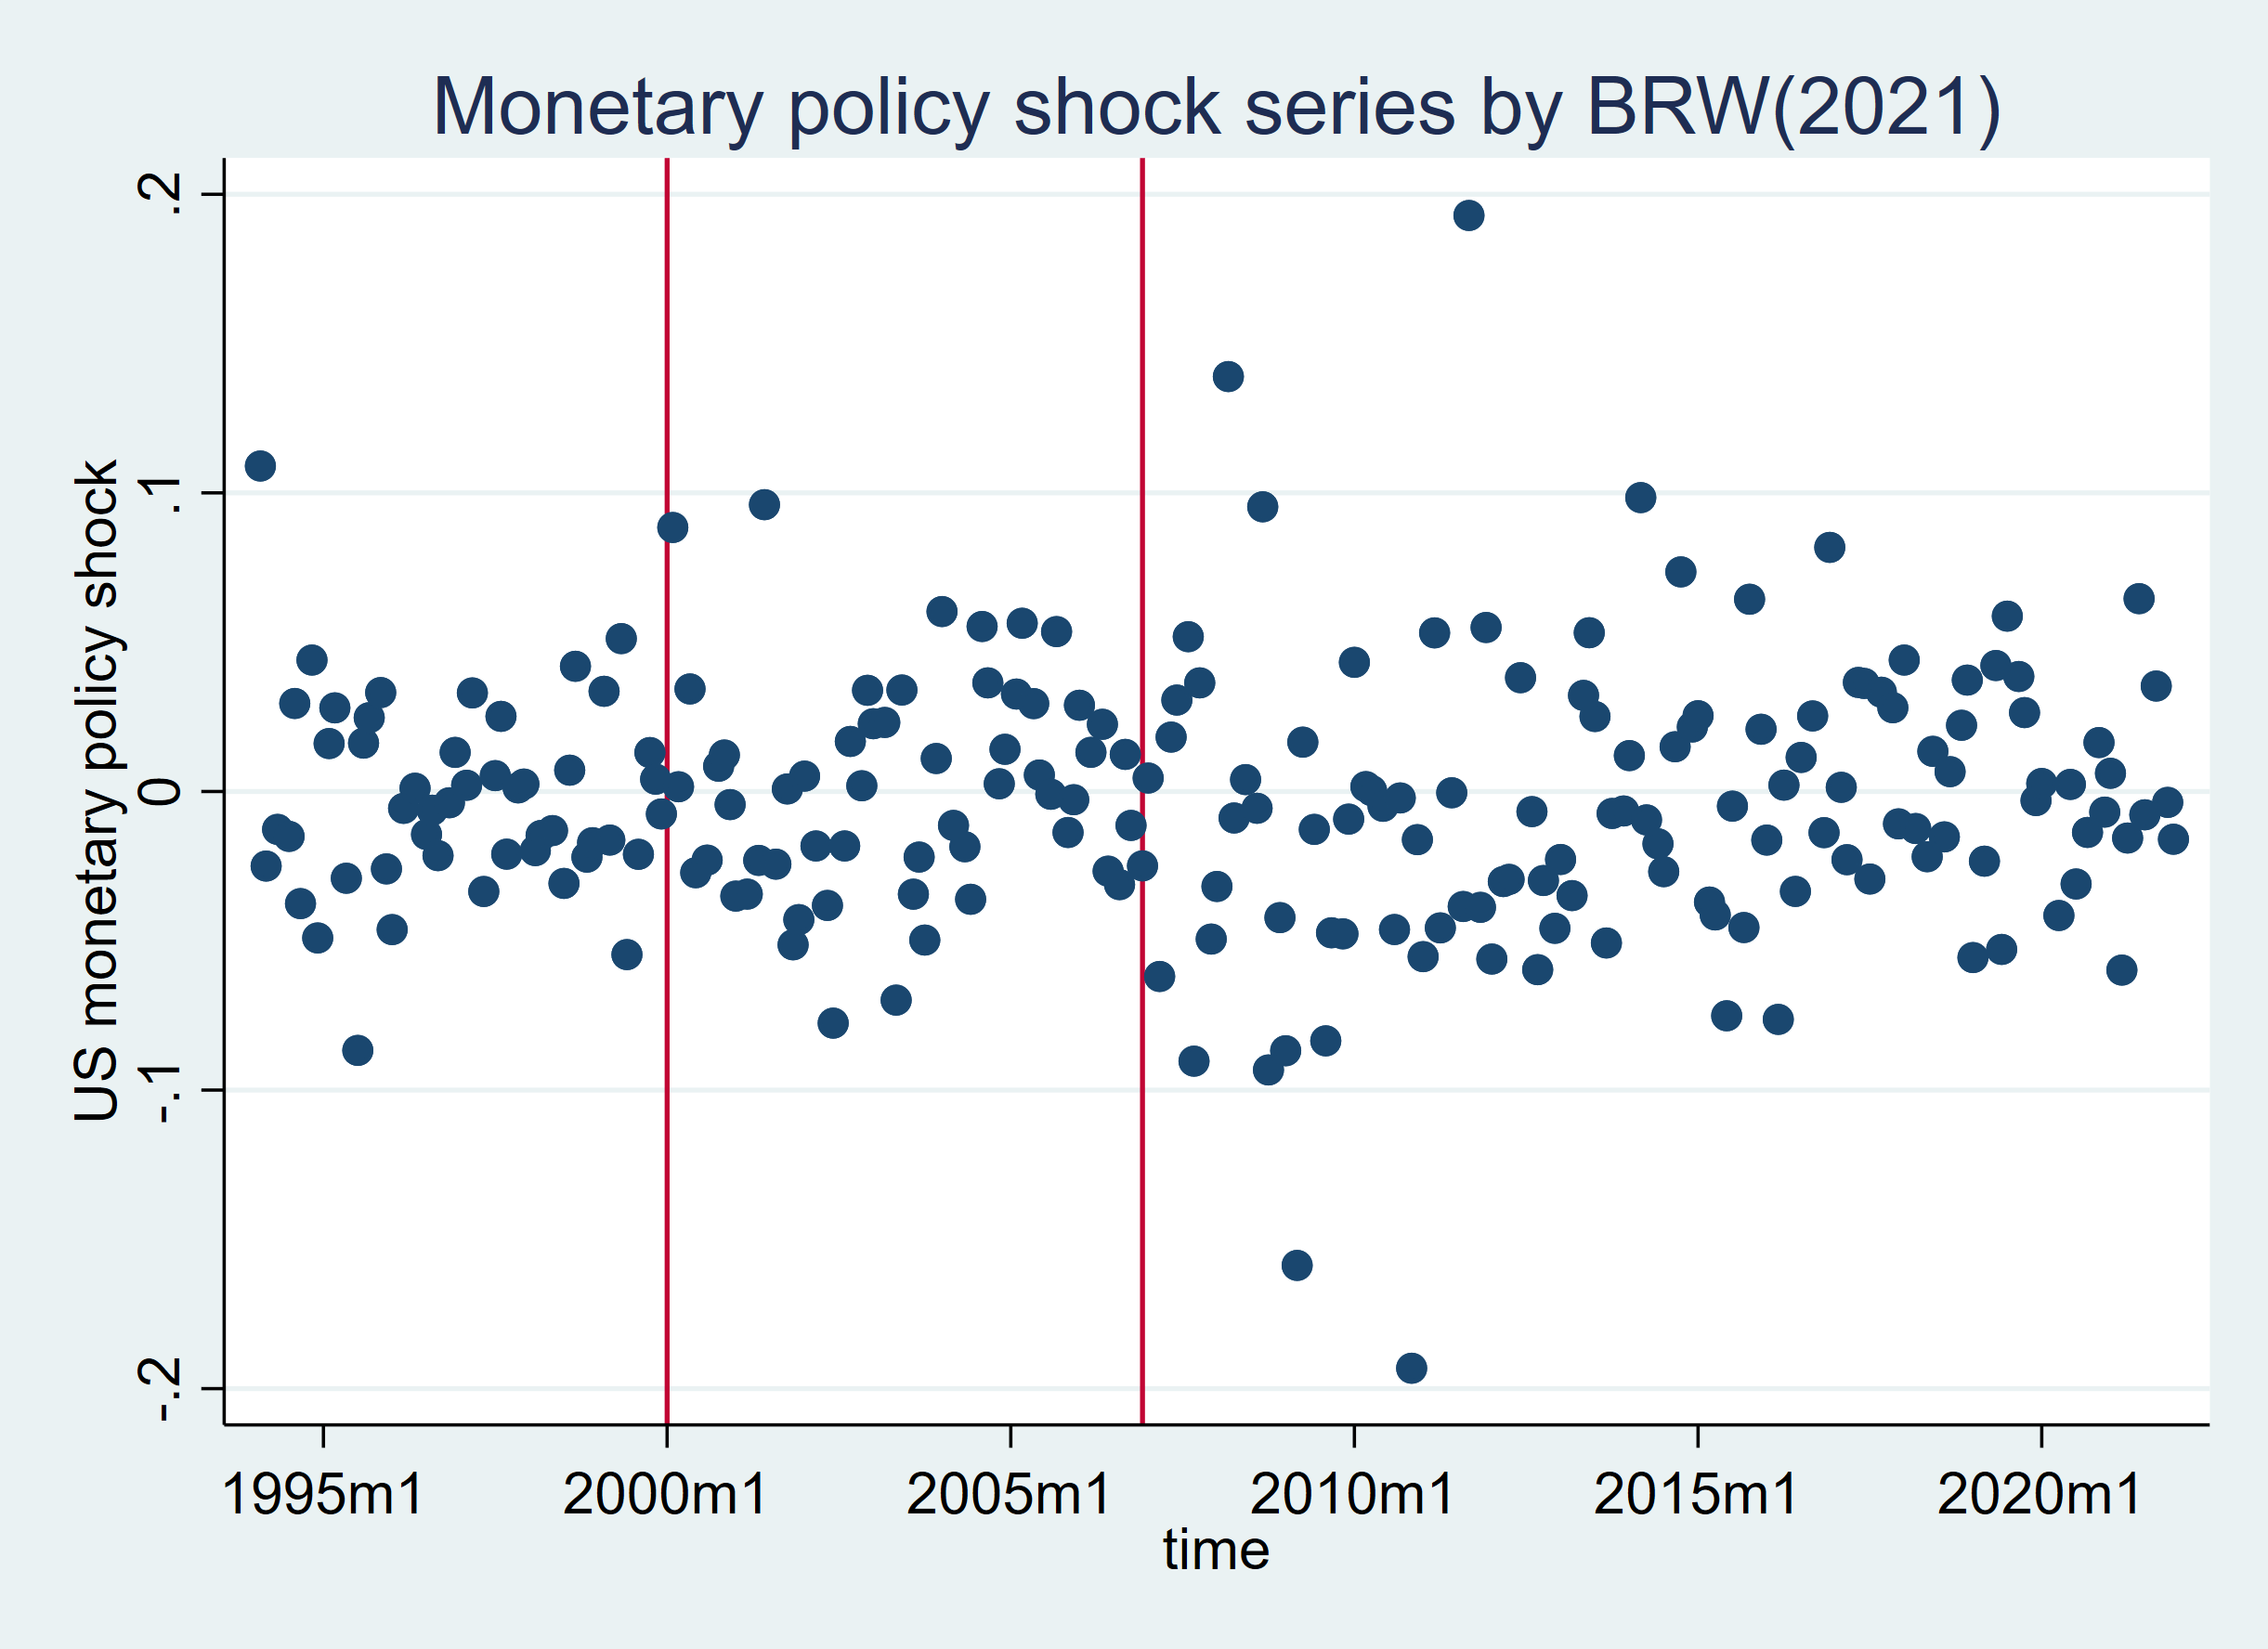
\includegraphics[width=0.9\textwidth]{latex/drafts/pic/BRW.png}
    \caption{\small US monetary policy shock: \cite{bu2021unified}}
    \label{fig: BRW}
\end{figure}


\subsection{Chinese firm-level data}

To investigate how exporters adjust their export prices in response to foreign monetary policy shocks, we merge the two disaggregated panel Chinese datasets: (1) the firm-level survey data and (2) the customs trade data between 2000 and 2006.

The source of Chinese firm-level production and financial information is the Annual Surveys of Industrial Enterprises in China (ASIE) conducted by the National Bureau of Statistics of China (NBSC). This database includes all state-owned enterprises and above-scale firms with more than 5 million RMB in annual sales. Between  and 2006,The datasets records 160,000 in 2000 to 300,000. Previous studies of the Chinese economy have widely used this database since it contains details about firms’ identification codes, ownership, industry type, and about 80 other accounting variables on the three major accounting statements (i.e., balance sheets, profit \& loss accounts, and cash flow statements). Among all that information, our research will focus on the variables related to two aspects: (1) firms' production costs and sales, including total wage payment, total operation inputs, and sales income, etc., and (2) firms' financial costs and liquidity conditions, including financial expense and interest payment, total and net working capital, cash holding, and others.

Manufacturing firms participating in international trade in the matched sample are uniquely identified by each observation's FRDM (legal entity) code and the survey year. To deal with reporting errors in the ASIE, we drop unsatisfactory observations referring to the criteria of \cite{fan2015credit} and \cite{brooks2021agglomeration}. We only keep firms that satisfy the following conditions: (1) a firm’s identification number cannot be missing and must be unique; (2) the key financial variables (such as total assets and sales income) cannot be missing;  (3) the total assets must be higher than the liquid assets and the total fixed assets; (4) the total assets must be higher than the liquid assets and the fixed assets; (5) the sales income cannot be negative; (6) the total liability cannot be negative; (7) the number of employees hired by a firm must not be less than 10.

\subsection{Customs trade data}

The second database we use is the transaction-level records from the General Administration of Customs of China (GACC). This dataset includes the most comprehensive information on all Chinese trade transactions, including each firm's import or export value denominated in US dollars, quantity, unit, product name and code, source or destination country, and the type of enterprises (e.g., state-owned, private, foreign-invested, and joint ventures), etc. In the raw data, each unique transaction refers to a firm-product-country-year pair. Of all customs information, each transaction's export value and quantity are of special interest because we can calculate the unit value by dividing the value by the quantity as an approximate measure of the export price, referring to the method of \cite{deloecker2012markups}. 

The categories of products in China's customs trade data are coded according to the Harmonized Coding and Description System (HS) of the World Customs Organization (WCO). The original data are subject to HS 8-digit classification. Since there were two major revisions of the HS system in 2002 and 2007, we aggregate HS8 product-level information to the HS6 level and then use conversion tables from the United Nations Trade Statistics to convert all codes into the older version of HS1996. We also drop unwanted observations referring to the standard of \cite{li2015exchange}: (1) products with inconsistent missing information of unit or quantity; (2) special product categories such as arms (HS2=93), antiques (HS2=97), and special categories (HS2=98 and 99); (3) transactions existing for only one year without any change over time.

We follow the standard procedure to match the identification codes based on the firms' contact information as in \cite{feenstra2014exports} to merge these firm-level survey data with customs trade data. Since we mainly focus on the short-term price response of Chinese exporters, we use the disaggregated monthly-level records to match high-frequency monetary policy shocks, a major difference between this article and previous literature using Chinese customs data. In Table \ref{tab.summary}, we provide summary statistics for firms' information and their export patterns in our matched sample. One notable point is that the distribution of firms' export value is skewed to the right long tail shape, with a few large exporters accounting for most of the trade value.

\begin{table}[htbp]
    \centering
    \caption{Summary statistics}
    \begin{threeparttable}
    \begin{tabular}{lccccc}
    \toprule
            &        Mean&          SD&         p50&         p25&         p75\\
    \midrule
    $\Delta P$        &        0.03&        0.42&        0.01&       -0.11&        0.17\\
    \# HS6 Products           &        6.29&       10.31&        3.00&        2.00&        7.00\\
    Export Value (*1000 RMB)    &   129580&   372029&    19709&     3890&    80525\\
    Sales (*1000 RMB)   &   160148&  1201262&    34910&    15350&    90852\\
    Employment     &      449&     1210&      197&       96&      418\\
    $Debt$              &        0.55&        0.26&        0.56&        0.37&        0.74\\
    $IE/L$               &        0.02&        0.04&        0.01&        0.00&        0.03\\
    $Liquid$       &        0.10 &        0.29 &        0.10 &       -0.07 &        0.28\\
    $\phi^{exp}$ (Export/Sales)         &        0.46&        0.38&        0.36&        0.07&        0.89\\
    $\phi^{imp}$ (Export/Inputs)               &        0.18&        0.30&        0.01&        0.00&        0.25\\
    \midrule
    Firm-year observations        &     \multicolumn{5}{c}{270271}      \\
    \bottomrule
    \end{tabular}
        \begin{tablenotes}
		\footnotesize
            \item Notes: This table shows the summary statistics of firms in the matched sample. The first row $\Delta P$ indicates monthly price changes, while all other rows describe annual-level firm variables.
	\end{tablenotes}
	\end{threeparttable}
    \label{tab.summary}
\end{table}

\subsection{Export price index}

The customs dataset contains disaggregated trade values denominated by US dollars and quantities for each HS6 product $h$, each firm $i$, to each country $c$, at time $t$, $V_{chit}$, and $Q_{chit}$. We first use the exchange rate between the US dollar and Chinese RMB to convert all trade values into RMB denominations. Then, we use the unit values as the proxy of export prices:

$$
P_{chit}=\frac{V_{chit}\cdot NER_{US,t}}{Q_{chit}}
$$

where $NER_{US,t}$ is the bilateral nominal exchange rate of US dollars in terms of RMB in month $t$. Because product categories are highly subdivided, we believe that the unit value is an ideal proxy for the transaction-level price. 

Using the above unit value price, we construct our firm-level Tornqvist price index using detailed information about the price of each product in each destination market following \cite{smeets2013estimating}. First, we aggregate the unit value to the firm-product level, which is the average price of product $h$ produced by firm $i$ weighted by the relative sales to each market $c$ at time $t$, $P_{hit}=\sum_c s_{c,hit} P_{chit}$, where the market-specific value share is $s_{c,hit}=V_{chit}/V_{hit}$. 

Second, we calculate the weighted average of the firm-product level price growth rate $\Delta_n \ln P_{hit} = P_{hit}- P_{hi(t-n)}$, for all product categories across $n$ periods: 

$$
\Delta_n P_{it} = \sum _{h} \frac{s_{h,i(t-n)}+s_{h,it}}{2} \Delta_n \ln P_{hit}
$$

where the product-specific value share is $s_{h,it}=V_{hit}/V_{it}$, and the effective weight is the average value of product weights at time $t$ and $t-n$. In the baseline monthly price regression, we set the time gap $n$ as 12 months (one year). This firm-level price growth rate $\Delta_{12m} P_{it}$ describes year-over-year changes for the average export price of a certain exporter, considering all adjustments to both product and market scopes. We will exclude observations with the annual growth rate of unit value in the top or bottom one percentile to avoid results being affected by extreme idiosyncratic factors other than monetary policy shocks.

\section{Empirical Results}

Our primary interest is to study the impacts of monetary policy shocks on export prices. This section describes our empirical specifications and shows how Chinese export prices adjust in response to unexpected US monetary policy shocks. We start from the baseline estimations of firm-level price response and then conduct robustness tests.

\subsection{Benchmark specification}

In the benchmark empirical test, we aggregate the export prices at the firm level and treat this as our starting point and benchmark. Although our export prices are at the firm-product-country level (namely, the transaction level), aggregation to firm-level price could avoid noises originating from too many dimensions. Apart from the global monetary policy shock, to control the firm-specific factors, we also add firm-fixed effect and other time-varying firm-level variables in the benchmark regression. Specifically, we consider the following specifications:

\begin{equation}
    \Delta \ln P_{it} = \alpha+\beta \cdot m_{t}+ \Gamma \cdot \textbf{Z}_{it-1}+\xi_{i}+\varepsilon_{it}
\end{equation}

where $\Delta \ln P_{it}$ represents the year-over-year export price change of firm $i$ at time $t$ (compared with the same month in last year), $m_t$ represents the unexpected monetary policy shock at time $t$. In the baseline regression, we use the measure of monetary policy shocks of \cite{bu2021unified}. Other alternative measures will also be employed in the robustness checks. $\textbf{Z}_{it-1}$ denotes lagged controls of firm-level time-variant variables. The two most important control variables are price changes in the previous period (controlling for price adjustment autocorrelation) and real sales income in the previous year (controlling for firm size). To control for unobserved firm heterogeneity, we include $\xi_{i}$ the firm-level fixed effect that captures any time-invariant factors for a given firm.

\subsection{Export price responses to monetary policy shocks}

The main results are displayed in Table \ref{tab.baseline}: on average, Chinese exporters will increase their prices in the short run, facing a contractionary US monetary policy shock. In column (1), we only include the monthly shock without other time-variant controls, and it is seen that one unit of US monetary policy shock (100 basis point increase in the 2-year US treasury yield rate) will induce an 18 $\%$ monthly increase in China's export prices by average. From columns (2)-(3), we observe that controlling other firm-level factors slightly reduces the magnitude of the price response, but the results are still significant. Columns (4)-(6) show the results when we aggregate the monthly sample to the annual level. In the annual sample, the dependent variable is annual price changes, and the monetary shock represents the sum of all the monthly shocks in that year. To summarize, we can observe a significant correlation between export price movements and unanticipated monetary policy shocks, with prices moving in the same direction as interest rates (i.e., a tighter monetary policy environment implies higher prices.)

\begin{table}[htbp]
    \centering
    \caption{Export price responses to US monetary policy shocks}
    \begin{threeparttable}
    \begin{tabular}{lcccccc}
        \toprule
        & (1)   & (2)   & (3)   & (4)   & (5)   & (6) \\
        & \multicolumn{3}{c}{Monthly $\Delta ln P_{it}$} & \multicolumn{3}{c}{Annual $\Delta ln P_{it}$}  \\
        \midrule
        $brw_t$   & 0.181*** & 0.145*** & 0.147*** & 0.136*** & 0.173*** & 0.173*** \\
              & (0.011) & (0.010) & (0.010) & (0.007) & (0.009) & (0.009) \\
        $\Delta ln P_{it-1}$ &       & 0.301*** & 0.299*** &       & -0.297*** & -0.298***  \\
              &       & (0.003) & (0.003) &       & (0.005) & (0.005) \\
        $Sales_{it-1}$ &       &       & -0.004*** &       &       &  0.004*\\
              &       &       & (0.001) &       &       &  (0.003)\\
        \midrule
        Firm FE & Yes   & Yes   & Yes   & Yes   & Yes   & Yes \\
        N     & 1100399 & 940015 & 917435 & 151542 & 96296 & 96296 \\
        \bottomrule
    \end{tabular}
        \begin{tablenotes}
            \footnotesize
            \item Notes: Robust standard errors clustered at the firm level;  *, **, and *** indicate significance at 10\%, 5\%, and 1\% levels. The dependent variables in columns (1)-(3) are changes in monthly price, while columns (4)-(6) are changes in annual price. All regressions include firm fixed effects.
	\end{tablenotes}
    \end{threeparttable}
    \label{tab.baseline}
\end{table}

Usually, there are eight scheduled FOMC meetings each year, each meeting with a corresponding policy shock. If there is no FOMC announcement in a month, then the shock in this month is zero.\footnote{This aggregation of monetary shocks is widely used in the literature, such as \cite{chari2021Taper}.} It turns out that the impact of the monetary shock is largely consistent with that of monthly regression.\footnote{As for the controlled variables, the coefficients are almost the opposite in the two versions; price changes display inertia in the short term and a pattern of mean regression in a relatively longer run, which is consistent with our intuition. Also, a firm with a bigger size tends to decrease its price in the short run while increasing the price in the longer run, which may be explained by the firm's price strategy and its market power. In this paper, we focus on the impact of global monetary policy shocks, so we will not explore this point in detail.} We also investigate the monthly dynamic responses and find that most of the adjustment takes place in the first six months, and the impact will gradually fade out within 12 months, indicating a short-term effect. The detailed results are displayed in Appendix \ref{tab.dynamic}.

\subsection{Robustness checks}

Our benchmark results are robust to many additional checks. First, we try \textit{alternative monetary policy shocks} in Table \ref{tab.altmps}. We first use the 30-minute high-frequency federal fund rate changes around the FOMC announcements to study the impact of conventional monetary policy shock, and then use the composite shock of \cite{nakamura2018high}, which is also a 30-minute high-frequency shock derived from the price changes of 2 federal fund rate futures and 3 Eurodollar futures around the FOMC announcement. This shock captures both the conventional monetary policy shock and the forward guidance. Moreover, we also employ the shock derived by \cite{guraynak2005actions}, who explicitly decompose an aggregate shock into the target and path part to represent conventional monetary policy shock and forward guidance, respectively. The data is obtained from \cite{acosta2022perceived} and is available on the author's personal website. The shocks mentioned above may have the concern of information effect (see the literature like \cite{nakamura2018high}, \cite{jarocinski2020deconstructing}, \cite{acosta2022perceived}, etc.). Namely, the policy action of the Fed may signal its private information about current and future economic fundamentals. So we also test the impact of the pure monetary policy shock of \cite{jarocinski2020deconstructing} who distinguish the pure policy shock from the information shock through the co-movement of treasury yield and stock prices. All of these measures suggest that a tightening shock will move export prices upward.

\begin{table}[htbp]
    \centering
    \caption{Alternative monetary policy shocks}
    \resizebox{\columnwidth}{!}{
    \begin{threeparttable}
    \begin{tabular}{lcccccccc}
        \toprule
        & (1)   & (2)   & (3)   & (4)   & (5)   & (6) & (7)   & (8) \\
        & \multicolumn{2}{c}{$\Delta$ FFR} & \multicolumn{2}{c}{Nakamura \& Steinsson}  & \multicolumn{2}{c}{Acosta} & \multicolumn{2}{c}{Jarocinski \& Karadi}\\
        \midrule
        $\Delta FFR_t$ & 0.029*** & 0.025***&       &        &       &       &       &  \\
              & (0.008) & (0.007)&       &        &       &       &       &  \\
        $NS_t$  &       &    & 0.152*** & 0.144***     &       &  \\
              &       &   & (0.009) & (0.009)       &       &  \\
        $Target^{US}_t$ &       &       &       &       & 0.002*** & 0.002*** &       &  \\
              &       &       &       &       & (0.000) & (0.000) &       &  \\
        $Path^{US}_t$  &       &       &       &       & 0.005*** & 0.004*** &       &  \\
              &       &       &       &       & (0.000) & (0.000) &       &  \\
        $MP_t$ &       &       &       &       &       &       & 0.045*** & 0.068*** \\
              &       &       &       &       &       &       & (0.006) & (0.006) \\
        $\Delta ln P_{it-1}$ &       & 0.299*** &       & 0.300*** &       & 0.299*** &       & 0.300*** \\
              &       & (0.003) &       & (0.003) &       & (0.003) &       & (0.003) \\
        $Sales_{it-1}$ &       & -0.005*** &       & -0.004*** &       & -0.005*** &       & -0.004*** \\
              &       & (0.001) &       & (0.001) &       & (0.001) &       & (0.001) \\
        \midrule
        Firm FE & Yes   & Yes   & Yes   & Yes   & Yes   & Yes   & Yes   & Yes \\
        N     & 1100399 & 917435 & 1100399 & 917435 & 1100399 & 917435 & 1100399 & 917435 \\
        \bottomrule
    \end{tabular}
        \begin{tablenotes}
            \footnotesize
            \item Notes: Robust standard errors clustered at the firm level;  *, **, and *** indicate significance at 10\%, 5\%, and 1\% levels. The dependent variables in all columns are changes in monthly price. Monetary policy shock measures in columns (1)-(2), (3)-(4), (5)-(6), (7)-(8) are from Fed fund rate changes, \cite{nakamura2018high}, \cite{acosta2022perceived}, and \cite{jarocinski2020deconstructing}, respectively. All regressions include firm fixed effects.
	\end{tablenotes}
    \end{threeparttable}
    }
    \label{tab.altmps}
\end{table}

Second, we adopt \textit{alternative ways of prices data aggregation} as in Table \ref{tab.altagg}. Firm-level price index adjustments give us an initial idea about price elasticity regarding monetary policy shocks. Here, we further use more disaggregated firm-product level prices and firm-product-country level prices as supplements. In the firm-product-country level regression, each transaction-level price is narrowly defined as the unit value of a certain product produced by a certain firm selling to a certain market. We add additional controls $RER_{ct}$, the bilateral real exchange rate between Chinese RMB and currency in the country $c$, and $RGDP_{ct}$, the real GDP of the source country deflated to the constant price level, which proxies for market demand. All results in those aggregation levels are consistent. 

Third, we limit our sample to \textit{single product firms}. In Table \ref{tab.single}, we repeat our baseline regressions on firms exporting only a single HS6 product within a given month. This test excludes any product switching effect affecting the firm-level price index. Although the sample size for single-product firms is much smaller, we observe similar price responses to monetary policy shocks. 

Fourth, we use \textit{alternative specifications with different standard error cluster levels and fixed effects}. Compared with our benchmark monthly regression, we also use a firm-year level cluster of standard error and include additional year fixed effect respectively, and the results are robust (see Table \ref{tab.altfe}).

Finally, we converted all export prices back to US dollars. Due to data limitations, we do not have specific information on the invoice currency used by each exporting company, but we know through anecdotal evidence that during the time period studied in this article (2000-2006), the vast majority of China's exports were denominated in RMB or US dollars. The results using U.S. dollar prices show that export price adjustments in response to monetary policy shocks are not sensitive to the invoicing currency (see Table \ref{tab.USD}).


\section{Mechanism}

In this section, we will explore the mechanism behind our benchmark findings. According to classical monetary policy theories, a tightening US monetary policy will push up global interest rates and incentivize households to consume less and deposit more, thus driving the shrinking of the global demand and decreasing product prices, contrary to our previous outcomes. Actually, apart from the demand-side story, the US monetary policy, as the main driver of the global financial cycle, will also affect China's export prices on the supply side through its impact on global borrowing cost and liquidity conditions. In the following parts, we will first decompose export price changes following the method of \cite{deloecker2012markups}into two parts: (1) the mark-up changes and (2) marginal cost changes. We will then display that only the marginal costs respond to the outside monetary shocks. Secondly, we further reveal that the marginal cost increase is mainly due to borrowing costs instead of other input costs, such as material costs, labor costs, and the cost of imported goods. We will also show that the deteriorating liquidity conditions further contribute to the uplift of export prices. In addition, we find that the impact of the US monetary policy on China's export prices is bigger, conditional on higher borrowing costs and tighter liquidity conditions, which further strengthens our argument that the supply-side effect is the dominant factor in shaping China's export prices.

\subsection{Decomposition of prices: markup vs marginal cost}

Firms are heterogeneous in their market power and profit margins, and therefore, their responses to global shocks may also be heterogeneous. Our data contains production firm-level information to decompose the price responses into markup adjustments and changes in marginal costs. This enables us to decompose exporters' price responses using their production characteristics.

Specifically, we can estimate the firm-level markup without direct prices and marginal cost measures using the structural assumptions of \cite{deloecker2012markups} and the GMM estimation method (\cite{brooks2021agglomeration}). We derive the firm-specific markup as the ratio of an input factor's output elasticity to its firm-specific factor payment share $\mu_{t}=\theta_{t}^{X}\left(\alpha_{t}^{X}\right)^{-1}$, where $\alpha_{t}^{X}$ is the share of expenditures on input X in total sales and $\theta^X_t$ denotes the output elasticity on input X. We apply the methodology of \cite{ackerberg2015} to address the endogeneity of inputs, assuming a third-order translog gross output production function. \footnote{Four production variables are logarithmic: real output value $y_t$, total employed persons $l_t$, real fixed assets at current value $k_t$, and real material inputs $m_t$. The function is in the form of $
    y_{t}= \beta_{k} k_{t}+\beta_{l} l_{t}+\beta_{i} m_{t}+\beta_{k 2} k_{t}^{2}+\beta_{l 2} l_{t}^{2}+\beta_{m 2} m_{t}^{2}+\beta_{k l} k_{ t} l_{t}+\beta_{k m} k_{t} m_{t}+\beta_{l m} l_{t} m_{t} + \beta_{k 3} k_{t}^{3}+\cdots+\omega_{t}+\epsilon_{t}.
$
All nominal values are deflated by deflators constructed as in \cite{brandt2012}.} The marginal cost, therefore, could be written as $MC_{it}=P_{it} / \mu_{it}$ and $\Delta ln(MC)_{it}= \Delta \ln P_{it} - \Delta \mu_{it}$ when $\mu \rightarrow 1$. 

With the decomposed series in hand, we replace the price changes with the markup and marginal cost changes separately in the benchmark regression. 

\begin{equation}
    \Delta \mu_{it} = \alpha +\beta \cdot brw_{t}+ \Gamma \cdot \textbf{Z}_{it-1}+\xi_{i}+\varepsilon_{it} \label{reg.markup}
\end{equation}

\begin{equation}
    \Delta \ln P_{it} = \alpha+\beta \cdot brw_{t}+ \gamma \cdot \Delta \mu_{it}+ \Gamma \cdot \textbf{Z}_{it-1}+\xi_{i}+\varepsilon_{i t} \label{reg.markup_int}
\end{equation}


The results of monthly data are displayed in Table \ref{tab.markup}. Column (1) directly uses Equation \ref{reg.markup}, and column (2) replaces the dependent variable with $MC_{it}$, indicating that the markup is almost unresponsive to the US monetary policy shocks, and only the marginal cost is adversely affected. In column (3), we use price changes as our dependent variable and further control the markup change as in \ref{reg.markup_int}. It is found that the impact of monetary policy shock on export prices is almost unchanged. In contrast, when we instead control the marginal cost changes in column (4), we find that the magnitude of the impact is substantially reduced by more than 75$\%$, further enhancing the dominating power of marginal cost. Columns (5)-(8) are the annual versions of the monthly regressions, and the results are qualitatively consistent with the monthly outcomes. In this version, we even spot that, although slightly, the markup is negatively affected by a tightening US shock. It is not difficult to understand this finding: exporting firms may depress their profit margin (namely, the markup) in recession business cycles to retain their market shares. 

\begin{table}[htbp]
    \centering
    \caption{Decomposition of prices: markup vs marginal cost}
    \resizebox{\columnwidth}{!}{
    \begin{threeparttable}
    \begin{tabular}{lcccccccc}
        \toprule
        & (1)   & (2)   & (3)   & (4)   & (5)   & (6) & (7)   & (8) \\
        & \multicolumn{4}{c}{Monthly sample} & \multicolumn{4}{c}{Annual sample}  \\
        \cline{2-5}  \cline{6-9}
        & $\Delta Markup_{it}$ & $\Delta ln(MC)_{it}$ & \multicolumn{2}{c}{$\Delta ln P_{it}$}  & $\Delta Markup_{it}$ & $\Delta MC_{it}$ & \multicolumn{2}{c}{$\Delta ln P_{it}$}\\
        \midrule
        $brw_t$   & -0.010 & 0.190*** & 0.149*** & 0.036*** & -0.017** & 0.174*** & 0.176*** & 0.084*** \\
              & (0.008) & (0.015) & (0.012) & (0.007) & (0.009) & (0.012) & (0.010) & (0.007) \\
        $\Delta Markup_{it}$&       &       & 0.004* &       &       &       &   0.007*    &  \\
              &       &       & (0.002) &       &       &       &   (0.004)    &  \\
        $\Delta MC_{it}$&       &       &       & 0.668*** &       &       &       &  0.472***\\
              &       &       &       & (0.004) &       &       &       &  (0.005)\\
        $\Delta ln P_{it-1}$&       &       & 0.280*** & 0.099*** &       &       &   -0.307*** & -0.163*** \\
              &       &       & (0.003) & (0.002) &       &       &   (0.005) & (0.004)  \\
        $Sales_{it-1}$ & -0.022*** & 0.019*** & -0.005*** & -0.018*** &  -0.022*** & 0.018*** & 0.006** & -0.009*** \\
              & (0.003) & (0.004) & (0.002) & (0.002) &  (0.002) & (0.003) & (0.003) & (0.002) \\
        \midrule
        Firm FE & Yes   & Yes   & Yes   & Yes   & Yes   & Yes   & Yes   & Yes \\
        N     & 830585 & 767768 & 665438 & 661680 & 110750 & 105330 & 81471 & 80831 \\
        \bottomrule
    \end{tabular}
        \begin{tablenotes}
            \footnotesize
            \item Notes: Robust standard errors clustered at the firm level;  *, **, and *** indicate significance at 10\%, 5\%, and 1\% levels. The dependent variables in columns (1), (2), (3)-(4) are changes in markup, marginal cost, and price in the monthly sample; the dependent variables in columns (5), (6), (7)-(8) are changes in markup, marginal cost, and price in the annual sample. All regressions include firm fixed effects.
	\end{tablenotes}
    \end{threeparttable}
    }
    \label{tab.markup}
\end{table}

\subsection{Borrowing cost and liquidity conditions}

The literature (\cite{RePEc:fip:fedkpr:y:2013:x:9}, \cite{georgiadis2016determinants} and \cite{miranda2020us} \footnote{“\textit{U.S. monetary policy shocks induce co-movements in the international financial variables that characterize the “Global Financial Cycle.” A single global factor that explains an important share of the variation of risky asset prices worldwide decreases significantly after a U.S. monetary tightening. Monetary contractions in the US led to significant deleveraging of global financial intermediaries, a global decline in domestic credit provision, strong retrenchments of international credit flows, and tightening of foreign financial conditions. Countries with floating exchange rate regimes are subject to similar financial spillovers.}” -- \cite{miranda2020us}}) has documented that contractionary U.S. monetary policy shocks will lead to the tightening of foreign financial conditions: interest rate increases, credit shrinking, bank deleveraging, and retrenchments of international credit flows. However, the impacts vary across the receiving country's characteristics, such as trade and financial integration, financial openness, exchange rate regime, financial market development, labor market rigidities, industry structure, and participation in global value chains. Even though the evidence above doesn't directly come from the data in China, we will show that China is not an exception and illustrate how these financial changes are related to export price adjustments. 

Actually, although China has strict capital control policies, \cite{prasad2007chinese} report that there have been huge capital inflows into China since 2003 that cannot be explained by trade surplus or foreign direct investments. Such international capital is referred to as “hot money.” Investors seek to earn short-term profits by arbitrating or speculating (\cite{kim2000fear}). Although various measures have been adopted by the authorities to restrict volatile international short-term capital flows that are speculative in nature, investors continue to circumvent the laws and regulations. \cite{martin2019china} indicate that over half of the hot money flown into China is over-reported or forged FDI. China is not fully isolated from hot money inflows because capital controls are not applied to all capital accounts transaction categories, and several are loosely managed (\cite{ping2004china}). So, we can treat China as a partially capital-free country, and the channels discussed in \cite{miranda2020us} still apply to China. Moreover, although China is found to be restrictive to portfolio flows, it is quite open to FDI inflows. \cite{lin2018foreign} reveal that there exists a trade credit channel through which FDI firms can propagate global liquidity shocks to the host economy despite its tight controls on non-FDI financial flows.
 
Therefore, whether through financial intermediaries, global asset prices, or trade provisions, all the previous literature implies that US tightening may increase Chinese firms' borrowing costs and harm their liquidity conditions. In light of this, we provide two hypotheses that link firms' export prices to global monetary policy shocks and the adjustment of financial conditions \footnote{To illustrate the channels more clearly, we built a stylized trade model augmented with monetary policy shock and financial frictions, which is displayed in the model section.}:

\begin{enumerate}
    \item \textbf{Global borrowing cost channel}. A tightening US monetary shock deteriorates the financing environment and increases the borrowing cost of firms, forcing them to offset this cost by lifting export prices.
    \item \textbf{Global liquidity channel}. A contractionary US monetary shock decreases the liquidity of export firms either through bank and trade credit shrinking or through the reduction of operational income, which induces firms to raise prices to alleviate liquidity constraints.
\end{enumerate}

In the previous section, we have already confirmed the cost-push effect of the US monetary policy shock. In this part, we further display that the borrowing costs are the main driver of the movement in aggregate costs. First, we will check whether and how borrowing costs and liquidity conditions of firms change with the monetary policy shocks:

\begin{equation}
    \Delta F_{it} = \alpha +\beta \cdot brw_{t}+ \Gamma \cdot \textbf{Z}_{it-1}+\xi_{i}+\varepsilon_{it} \label{reg.liquid}
\end{equation}

where $F$ is the firm's borrowing cost or liquidity. Here we aggregate US shock at the year level to be consistent with the frequency of dependent variables.

The results can be seen in Table \ref{tab.liquid}. In Columns (1)-(4), we directly regress the annual change in financial cost on monetary policy shocks with the control of previous firm size $Sales_{it-1}$ and debt to asset ratio $Debt$. We use four indicators to measure the change in borrowing cost: the change of interest expenditure to the total liability $\Delta IE/L$, the change of interest expenditure to the total current liability $\Delta IE/L$, the change of financial expenditure (including the interest rate expenditure and other borrowing-related financial costs) to the total liability $\Delta FN/L$, and the change of financial expenditure to the total current liability $\Delta FN/CL$. All of these variables are constructed by the firm-level survey data described previously. It turns out that the borrowing cost will significantly move up after a tightening US shock. For example, as in Column (1), one unit of positive US monetary policy shock (100 basis points increase in the US 2-Y treasury yield) will raise the ratio of interest expenditure to total liability $\Delta IE/L$ by 0.2 $\%$. 

In columns (5)-(8), we use the same specification as the former four columns and replace borrowing cost changes with the changes in liquidity conditions, measured by the change of working capital to total asset $\Delta WC$, the change of the net liquid asset (liquid asset minus liquid liability) to total asset $\Delta Liquid$, the change of cash to total asset $\Delta Cash$, and the change of accounts receivable to total sales $\Delta Arec$ (i.e. trade credit). Similarly, the data of these variables are also from the firm-level survey data. It is found that the US monetary policy shocks severely impact the liquidity conditions of China's exporting firms. For instance, one unit of positive US monetary policy shock (100 basis points increase in the US 2-Y treasury yield) will reduce the cash ratio by 0.7 $\%$ on average. The above results verified our previous assumptions that the US monetary policy shock can affect China's export prices through borrowing costs and liquid channels.

\begin{table}[htbp]
    \centering
    \caption{Borrowing cost channel and liquidity channel}
    \resizebox{\columnwidth}{!}{
    \begin{threeparttable}
    \begin{tabular}{lcccccccc}
        \toprule
        & (1)   & (2)   & (3)   & (4)   & (5)   & (6) & (7)   & (8) \\
        & $\Delta IE/L$ & $\Delta IE/L$ & $\Delta FN/L$ & $\Delta FN/CL$ & $\Delta WC$  & $\Delta Liquid$ & $\Delta Cash$ & $\Delta Arec$ \\
        \midrule
        $brw_t$   & 0.002*** & 0.004*** & 0.002*** & 0.004*** & -0.005*** & -0.021*** & -0.007*** & -0.004** \\
              & (0.000) & (0.001) & (0.001) & (0.001) & (0.002) & (0.002) & (0.002) & (0.002) \\
        $Sales_{it-1}$ & -0.001*** & -0.002*** & -0.003*** & -0.004*** & -0.009*** & -0.000 & -0.001*** & 0.059*** \\
              & (0.000) & (0.000) & (0.000) & (0.000) & (0.000) & (0.001) & (0.000) & (0.001) \\
        $Debt_{it-1}$ & 0.045*** & 0.052*** & 0.080*** & 0.089*** & -0.105*** & 0.599*** & -0.005*** & -0.053*** \\
              & (0.001) & (0.001) & (0.001) & (0.001) & (0.002) & (0.002) & (0.002) & (0.002) \\
        \midrule
        Firm FE & Yes   & Yes   & Yes   & Yes   & Yes   & Yes   & Yes   & Yes \\
        N     & 1081803 & 1056283 & 1081803 & 1056283 & 1090620 & 1090620 & 1090620 & 1090620 \\
        \bottomrule
    \end{tabular}
        \begin{tablenotes}
            \footnotesize
            \item Notes: Robust standard errors clustered at the firm level;  *, **, and *** indicate significance at 10\%, 5\%, and 1\% levels. The dependent variables in columns (1)-(4) are changes in interest expense over the total liability ratio, interest expense over the current liability ratio, total financial expense over the total liability ratio, and total financial expense over the current liability ratio, respectively. The dependent variables in columns (5)-(8) are changes in working capital over total asset ratio, net liquidity asset over total asset ratio, cash over total asset ratio, and accounts receivable over sales ratio, respectively. All regressions include firm fixed effects.
	\end{tablenotes}
    \end{threeparttable}
    }
    \label{tab.liquid}
\end{table}

Furthermore, we have done an additional analysis to rule out the confounding effects of adjusting other costs. The results are shown in Table \ref{tab.other}. In columns (1)-(2), we regress the change of input costs to sales and the change of wage payments to sales on the monetary shock, respectively, and the results are insignificant. Moreover, we also incorporate the interaction term of monetary shock and the two variables into the benchmark regression as Equation \ref{reg.int}. 

\begin{equation}
    \Delta F_{it} = \alpha +\beta_1 \cdot brw_{t} +\beta_2 \cdot brw_{t} \times X_{it}+ \Gamma \cdot \textbf{Z}_{it-1}+\xi_{i}+\varepsilon_{it} \label{reg.int}
\end{equation}

\begin{table}[htbp]
    \centering
    \caption{Discussion about other production costs}
    \resizebox{\columnwidth}{!}{
    \begin{threeparttable}
    \begin{tabular}{lccccccc}
        \toprule
        & (1)   & (2)   & (3)   & (4)   & (5)   & (6) & (7) \\
        & $\Delta Input/Sales$ & $\Delta Wage/Sales$ & \multicolumn{5}{c}{$\Delta ln P_{it}$}\\
        \midrule
        $brw_t$   & 0.403 & -0.164 & 0.142*** & 0.159*** & 0.154*** & 0.159*** & 0.147*** \\
              & (0.263) & (0.135) & (0.011) & (0.013) & (0.014) & (0.024) & (0.010) \\
        $brw_t \times Input/Sales $ &       &       & 0.007 &       &       &       &  \\
              &       &       & (0.005) &       &       &       &  \\
        $brw_t \times Wage/Sales $ &       &       &       & -0.108 &       &       &  \\
              &       &       &       & (0.078) &       &       &  \\
        $brw_t \times \phi^{imp}_t$ &       &       &       &       & -0.027 &       &  \\
              &       &       &       &       & (0.032) &       &  \\
        $brw_t \times \phi^{exp}_t$  &       &       &       &       &       & -0.019 &  \\
              &       &       &       &       &       & (0.032) &  \\
        $brw_t \times \phi^{trade}_t$ &       &       &       &       &       &       & -0.000 \\
              &       &       &       &       &       &       & (0.000) \\
        $Debt_{it_1}$ & 0.436** & 0.241 &       &       &       &       &  \\
              & (0.180) & (0.162) &       &       &       &       &  \\
        $\Delta ln P_{it-1}$ &       &       & 0.299*** & 0.299*** & 0.299*** & 0.299*** & 0.299*** \\
              &       &       & (0.003) & (0.003) & (0.003) & (0.003) & (0.003) \\
        $Sales_{it-1}$ &  1.075*** & -0.044   & -0.004*** & -0.004*** & -0.004*** & -0.004*** & -0.004*** \\
              &  (0.262) & (0.187) & (0.001) & (0.001) & (0.001) & (0.001) & (0.001) \\
        \midrule
        Firm FE & Yes   & Yes   & Yes   & Yes   & Yes   & Yes   & Yes \\
        N     & 1090620 & 1090620 & 917435 & 917435 & 917435 & 917435 & 917435 \\
        \bottomrule
    \end{tabular}
        \begin{tablenotes}
            \footnotesize
            \item Notes: Robust standard errors clustered at the firm level;  *, **, and *** indicate significance at 10\%, 5\%, and 1\% levels. The dependent variables in columns (1)-(2) are changes in intermediate input cost over sales ratio and wage expense over sales ratio, respectively. The dependent variables in columns (3)-(7) are changes in monthly price. All regressions include firm fixed effects.
	\end{tablenotes}
    \end{threeparttable}
    }
    \label{tab.other}
\end{table}

In columns (3)-(4), the results are not significant either, which suggests that the shifts in these two types of shocks are not the reason for export price adjustments. It is also possible that the prices of imported goods may also increase, affecting China's export prices. To invalidate this assumption, we include the interaction term of monetary shock and import intensity $\phi^{imp}$ (the ratio of import to sales) in column (5), and the coefficients are not significant. Similarly, in columns (6)-(7), we also check that export intensity $\phi^{exp}$ (the ratio of export to sales) and trade intensity $\phi^{trade}$ (the ratio of import and export to sales) are not related to the impact of the US monetary shock on China's export prices.

Moreover, we also find that the impact of the US monetary policy shock on China's export prices is non-linear: the effect of monetary policy shocks is bigger for firms with higher borrowing costs and tighter credit conditions. From Table \ref{tab.non-linearity}, we can see that the coefficients of the interaction term of monetary shock and borrowing cost are positive and significant, and that of liquidity measures are most negative and significant (3 out of 4 measures). Need to mention that to avoid the reverse causality problem of price changes with borrowing cost and liquidity conditions, as all of these variables are at the firm level, we aggregate the firm-level borrowing costs and liquidity conditions at the industry level. These results further strengthen the connection between firms' export prices and borrowing costs or liquidity conditions in the presence of foreign monetary policy shocks.

\begin{table}[htbp]
    \centering
    \caption{Non-linearity of borrowing cost channel and liquidity channel}
    \resizebox{\columnwidth}{!}{
    \begin{threeparttable}
    \begin{tabular}{lcccccccc}
        \toprule
        & (1)   & (2)   & (3)   & (4)   & (5)   & (6)   & (7)   & (8) \\
    \midrule
    $brw_t$ & 0.107*** & 0.109*** & 0.087*** & 0.092*** & 0.351*** & 0.236*** & 0.510*** & 0.129*** \\
          & (0.017) & (0.017) & (0.033) & (0.031) & (0.097) & (0.022) & (0.082) & (0.025) \\
    $brw_t \times IE/L_{st}$ & 6.580*** &       &       &       &       &       &       &  \\
          & (1.977) &       &       &       &       &       &       &  \\
    $brw_t \times IE/CL_{st}$ &       & 5.415*** &       &       &       &       &       &  \\
          &       & (1.701) &       &       &       &       &       &  \\
    $brw_t \times FN/L_{st}$ &       &       & 4.203** &       &       &       &       &  \\
          &       &       & (2.112) &       &       &       &       &  \\
    $brw_t \times FN/CL_{st}$ &       &       &       & 3.466** &       &       &       &  \\
          &       &       &       & (1.768) &       &       &       &  \\
    $brw_t \times WC_{st}$ &       &       &       &       & -0.331** &       &       &  \\
          &       &       &       &       & (0.159) &       &       &  \\
    $brw_t \times Liquid_{st}$ &       &       &       &       &       & -1.137*** &       &  \\
          &       &       &       &       &       & (0.270) &       &  \\
    $brw_t \times Cash_{st}$ &       &       &       &       &       &       & -2.226*** &  \\
          &       &       &       &       &       &       & (0.498) &  \\
    $brw_t \times Arec_{st}$ &       &       &       &       &       &       &       & 0.167 \\
          &       &       &       &       &       &       &       & (0.218) \\
    $\Delta ln P_{it-1}$ & 0.299*** & 0.299*** & 0.299*** & 0.299*** & 0.299*** & 0.299*** & 0.299*** & 0.299*** \\
          & (0.003) & (0.003) & (0.003) & (0.003) & (0.003) & (0.003) & (0.003) & (0.003) \\
    $Sales_{it-1}$ & -0.004*** & -0.004*** & -0.004*** & -0.004*** & -0.004*** & -0.004*** & -0.004*** & -0.004*** \\
          & (0.001) & (0.001) & (0.001) & (0.001) & (0.001) & (0.001) & (0.001) & (0.001) \\
    \midrule
    Firm FE & Yes   & Yes   & Yes   & Yes   & Yes   & Yes   & Yes   & Yes \\
    N     & 917435 & 917435 & 917435 & 917435 & 917435 & 917435 & 917435 & 917435 \\
        \bottomrule
    \end{tabular}
        \begin{tablenotes}
            \footnotesize
            \item Notes: Robust standard errors clustered at the firm level;  *, **, and *** indicate significance at 10\%, 5\%, and 1\% levels. The interaction terms in columns (1)-(8) are the industry-level average interest expense over the total liability ratio, interest expense over the current liability ratio, total financial expense over the total liability ratio, total financial expense over the current liability ratio, working capital over total asset ratio, net liquidity asset over total asset ratio, cash over total asset ratio, and accounts receivable over sales ratio. All regressions include firm fixed effects.
	\end{tablenotes}
    \end{threeparttable}
    }
    \label{tab.non-linearity}
\end{table}

\subsection{Ordinary trade vs processing trade}

Some exporters may be registered as "processing trade. That is, importing raw materials and intermediate inputs from abroad in bond for domestic processing and re-export\footnote{ Ordinary trade firms account for more than 2/3 of the total observations in our sample. Therefore, the pricing patterns based on ordinary trade should dominate the overall Chinese trade.}. Processing trade contracts is more fixed than that of ordinary trade. Moreover, financial frictions could affect firms' choice between processing and ordinary trade, which is a choice of production technology and its position in global supply chains. Therefore, processing trade could also implicitly imply some firm characteristics related to its market power (\cite{manova2016firms}). Due to the sorting mechanism, firms participating in more processing trade usually have less borrowing needs and are less constrained by liquidity conditions. So, if the borrowing cost and liquidity channels hold, we expect that the price response for the processing trader should be smaller than that of the ordinary traders. 

We provide evidence about the price response patterns for ordinary trade compared with processing trade in Table \ref{tab.process}. Columns (1)-(2) only include the sample of ordinary trade transactions. In columns (3)-(4), we instead show the results using only processing trade transactions. In columns (5)-(6), we use the processing trade intensity as the interaction term to study the difference between processing and ordinary trade. In practice, in the firm-product level sample, we create a processing trade dummy, which takes the value of 1 when a transaction belongs to processing trade and 0 when it belongs to ordinary trade \footnote{When aggregating to a firm-level sample, we compute the processing trade intensity as the average number of processing trade products weighted by the export value.}. All these results show that the impact of US shock on processing traders is much smaller than that of ordinary traders, which verifies our conjecture and further reinforces our proposed mechanisms.

\begin{table}[h]
    \centering
    \caption{Ordinary trade vs processing trade}
    \begin{threeparttable}
    \begin{tabular}{lcccccc}
        \toprule
        & (1)   & (2)   & (3)   & (4)   & (5)   & (6) \\
          & \multicolumn{2}{c}{Ordinary trade}  & \multicolumn{2}{c}{Processing trade} & \multicolumn{2}{c}{Comparison}\\
        \midrule
        $brw_t$   & 0.201*** & 0.186*** & 0.098*** & 0.065*** & 0.225*** & 0.185*** \\
              & (0.018) & (0.019) & (0.019) & (0.016) & (0.016) & (0.016) \\
        $brw_t \times process_{it}$ &       &       &       &       & -0.102*** & -0.085*** \\
              &       &       &       &       & (0.024) & (0.023) \\
        $\Delta ln P_{it-1}$ &       & 0.190*** &       & 0.473*** &       & 0.299*** \\
              &       & (0.003) &       & (0.005) &       & (0.003) \\
        $Sales_{it-1}$ &       & -0.004* &       & -0.009*** &       & -0.004*** \\
              &       & (0.002) &       & (0.002) &       & (0.001) \\
        Firm FE & Yes   & Yes   & Yes   & Yes   & Yes   & Yes \\
        N     & 499418 & 391336 & 283952 & 242587 & 1100399 & 917435 \\
        \bottomrule
    \end{tabular}
        \begin{tablenotes}
            \footnotesize
            \item Notes: Robust standard errors clustered at the firm level;  *, **, and *** indicate significance at 10\%, 5\%, and 1\% levels. The dependent variables in columns (1)-(3) are changes in monthly price denominated in the US dollar, while columns (4)-(6) are changes in annual price denominated in the US dollar. All regressions include firm fixed effects.
	\end{tablenotes}
    \end{threeparttable}
    \label{tab.process}
\end{table}

\subsection{Alternative explanations}

In addition to the channels mentioned above, there might be two other potential explanations for the export price increase after a tightening US monetary shock:

(1) \textbf{Demand shift} 

A tightening global monetary shock will induce a recession business cycle, which might make Chinese exports more competitive because some Chinese products are cheaper and of lower quality than similar ones from other developed countries. The idea is similar to the concept of Giffen goods: the prices of inferior goods increase when people's incomes drop. However, in Table \ref{tab.rauch}, we find that the prices of homogeneous goods also increase even more. These goods have little differences in quality and can't be treated as Giffen products. Thus, this explanation does not suit our benchmark findings.

\begin{table}[htbp]
    \centering
    \caption{Homogeneous good vs differentiated good}
    \resizebox{\columnwidth}{!}{
    \begin{threeparttable}
    \begin{tabular}{lcccccccc}
        \toprule
        & (1)   & (2)   & (3)   & (4)   & (5)   & (6)   & (7)   & (8) \\
        & \multicolumn{4}{c}{Conservative classification} & \multicolumn{4}{c}{Liberal classification} \\
        \midrule
        $brw_t$   & 0.170*** & 0.126*** & 0.149*** & 0.114*** & 0.168*** & 0.124*** & 0.148*** & 0.115*** \\
          & (0.011) & (0.011) & (0.012) & (0.012) & (0.012) & (0.011) & (0.013) & (0.012) \\
        $brw_t \times ToE_{it} $ & 0.152 & 0.112 &       &    & 0.263*** & 0.242***    &       &  \\
          & (0.128) & (0.125) &       &      & (0.086) & (0.082)     &       &  \\
        $brw_t \times Ref_{it} $ &       &       & 0.208*** & 0.125*** &       &    & 0.167*** & 0.082*** \\
          &       &       & (0.033) & (0.032) &       &         & (0.031) & (0.030)\\
        $\Delta ln P_{it-1}$ &       & 0.298*** &       & 0.298*** &       & 0.298*** &       & 0.298*** \\
          &       & (0.003) &       & (0.003) &       & (0.003) &       & (0.003) \\
        $Sales_{it-1}$ &       & 0.004*** &       & 0.004*** &       & 0.004*** &       & 0.004*** \\
          &       & (0.001) &       & (0.001) &       & (0.001) &       & (0.001) \\
    \midrule
    Firm FE & Yes   & Yes   & Yes   & Yes   & Yes   & Yes   & Yes   & Yes \\
    N     & 1014106 & 850174 & 1014106 & 850174 & 1014106 & 850174 & 1014106 & 850174 \\
        \bottomrule
    \end{tabular}
        \begin{tablenotes}
            \footnotesize
            \item Notes: Robust standard errors clustered at the firm level;  *, **, and *** indicate significance at 10\%, 5\%, and 1\% levels. The variables "ToE" and "Ref" represent the value share of goods traded on an organized exchange and the value share of reference-priced goods of firm $i$. Columns (1)-(4) use the "conservative" classification, while columns (5)-(8) use the "liberal" classification, both referring to \cite{rauch1999networks}. All regressions include firm fixed effects.
	\end{tablenotes}
    \end{threeparttable}
    }
    \label{tab.rauch}
\end{table}

(2) \textbf{Exchange rate pass-through} 

Classical monetary and exchange rate literature suggests that a tightening US monetary shock will cause the depreciation of the currencies in other countries. Moreover, many exchange-rate pass-through papers have revealed that exchange-rate depreciation will increase export prices denominated in domestic currency. However, this explanation is not likely to be the main reason for the price response. we have controlled the change of bilateral real exchange rate as in the annual firm-product-country level regression (Columns (4)-(6) of Table \ref{tab.altagg}), and the results are robust. Conceptually, due to the existence of capital control in China, interest parity does not always hold for China, which implies that the effect of the interest rate should be separated from the exchange rate pass-through.

\newpage
\section{More Discussion}

\subsection{EU monetary policy shocks}

Apart from the spillover effect of US monetary policy shock, recent literature (see \cite{ca2020monetary}, \cite{corsetti2021exchange} and \cite{miranda2022tale}, etc.) indicates that the monetary shock of the European Central Bank (ECB) also has a substantial effect on global financial conditions and real economic activities. Using the same specification as our benchmark regression, we explore how China's export prices respond to the ECB monetary shocks in Table \ref{tab.EU}. In Column (1)-(3), we use the target shock from \cite{miranda2022tale} \footnote{Using the approach of \cite{swanson2021measuring}, \cite{miranda2022tale} decomposes the ECB monetary shock into three components: the target, path and lsap part, which reflects unexpected policy rate change, forward guidance and Large-scale asset purchasing respectively. In our main sample (2000-2006), traditional monetary policy dominates, so here we only use the target shock.}. To avoid the confounding effect stemming from the central bank information effect, we also use the pure monetary policy shock of \cite{jarocinski2020deconstructing} in Column (4)-(6). It is seen that, unlike the reaction to the US shock, Chinese export prices barely move in response to the European monetary policy shocks. One unit of tightening target shock (increase 1-month OIS rate by 100 basis points) will decrease China's export prices by only 0.1$\%$ (see Column (3)). Also, when we use the pure monetary policy shock of \cite{jarocinski2020deconstructing}, this impact even becomes insignificant (see Column (6)). Our finding is consistent with the conclusion in the literature (like \cite{ca2020monetary}, \cite{corsetti2021exchange} and \cite{miranda2022tale}, etc.) that the spillover effect of ECB shock is less powerful than that of the Fed. This is easy to understand because the dominant role of the US dollar along with the intensive integration of the global financial market confers the US monetary policy a special role to drive the global financial cycle (GFC) (\cite{miranda2020us}). Another possible explanation is that, in most of our sample period, China's exchange rate is fixed to the US dollar, and a substantial proportion of the transactions may invoiced in the US dollar, which may augment the impact of US shock on China's export prices. 

\begin{table}[htbp]
    \centering
    \caption{Export price responses to EU monetary policy shocks}
    \begin{threeparttable}
    \begin{tabular}{lcccccc}
        \toprule
        & (1)   & (2)   & (3)   & (4)   & (5)   & (6) \\
        & \multicolumn{3}{c}{Miranda-Agrippino \& Nenova} & \multicolumn{3}{c}{Jarocinski \& Karadi}  \\
        \midrule
        $m^{EU}_t$ & -0.002*** & -0.001*** & -0.001*** & -0.050*** & 0.002 & -0.002 \\
              & (0.000) & (0.000) & (0.000) & (0.011) & (0.011) & (0.011)\\  
        $\Delta ln P_{it-1}$ &       & 0.301*** & 0.300*** &       & 0.301*** & 0.300*** \\
              &       & (0.003) & (0.003) &       & (0.005) & (0.005) \\
        $Sales_{it-1}$ &       &       & -0.004*** &       &       & -0.004*** \\
              &       &       & (0.001) &       &       & (0.001) \\
        \midrule
        Firm FE & Yes   & Yes   & Yes   & Yes   & Yes   & Yes \\
         N     & 1100399 & 940015 & 917435 & 1100399 & 940015 & 917435 \\
        \bottomrule
    \end{tabular}
        \begin{tablenotes}
            \footnotesize
            \item Notes: Robust standard errors clustered at the firm level;  *, **, and *** indicate significance at 10\%, 5\%, and 1\% levels. Monetary policy shocks here are from the European Central Bank. The shock in columns (1)-(3) are obtained from \cite{miranda2022tale}, while columns (4)-(6) are  from \cite{jarocinski2020deconstructing}. All regressions include firm fixed effects.
	\end{tablenotes}
    \end{threeparttable}
    \label{tab.EU}
\end{table}

\subsection{Alternative time horizon}

Our monthly sample period covers 84 months from January 2000 to December 2006, when the RMB was pegged with the US dollar before July 2005. After that, China began to target a basket of currency, allowing the fluctuation of the exchange rate to the US dollar. To investigate whether the export responses to global monetary shocks vary across exchange rate regimes, we split the whole sample into two parts: the fixed regime (Jan 2000 - June 2005) and the floating regime (July 2005 - Dec 2006) and redo the benchmark regression separately over the two sub-samples. In Table \ref{tab.regime}, we can see that the coefficient in the fixed regime is around 0.14 (Column 3), while it drops to 0.08 in the floating regime (Column 6). This indicates that the floating exchange serves as a buffer to external monetary shocks, but the spillover effect is not absolutely isolated, which is consistent with the conclusion in the literature, like \cite{shambaugh2004effect}, \cite{klein2012exchange}, \cite{georgiadis2016determinants}, \cite{dedola2017if}, etc. Therefore, the policy implication is that a more floating and flexible exchange rate regime can be adopted to mitigate the adverse impact of foreign monetary policy shocks.

\begin{table}[htbp]
    \centering
    \caption{Exchange rate regime shift: before and after July 2005}
    \begin{threeparttable}
    \begin{tabular}{lcccccc}
        \toprule
        & (1)   & (2)   & (3)   & (4)   & (5)   & (6) \\
        & \multicolumn{3}{c}{Fixed regime: before July 2005} & \multicolumn{3}{c}{Floating regime: after July 2005}  \\
        \midrule
        $brw_t$   & 0.189*** & 0.138*** & 0.138*** & 0.031 & 0.108*** & 0.080*** \\
              & (0.012) & (0.012) & (0.012) & (0.022) & (0.023) & (0.023) \\
        $\Delta ln P_{it-1}$ &       & 0.288*** & 0.287*** &       & 0.186*** & 0.182*** \\
              &       & (0.003) & (0.003) &       & (0.004) & (0.004) \\
        $Sales_{it-1}$ &       &       & 0.000 &       &       & -0.025*** \\
              &       &       & (0.002) &       &       & (0.004) \\
        \midrule
        Firm FE & Yes   & Yes   & Yes   & Yes   & Yes   & Yes \\
        N     & 708254 & 609726 & 594891 & 389776 & 328076 & 320432 \\
        \bottomrule
    \end{tabular}
        \begin{tablenotes}
            \footnotesize
            \item Notes: Robust standard errors clustered at the firm level;  *, **, and *** indicate significance at 10\%, 5\%, and 1\% levels. Columns (1)-(3) cover the period from January 2000 to July 2005, while columns (4)-(6) cover the period from August 2005 to December 2006. All regressions include firm fixed effects.
	\end{tablenotes}
    \end{threeparttable}
    \label{tab.regime}
\end{table}


\newpage
\section{Model}

In this section, we construct a partial equilibrium model to show how exporting firms' behaviors respond to a global monetary contraction, which illustrates the mechanism is related to borrowing cost increases and liquidity constraints.  \footnote{A general equilibrium model will not alter the direction of the impact of global monetary policy shocks.} The model builds on the heterogeneous-firm trade model of \cite{melitz2003impact} and \cite{manova2013credit}, and we further incorporate the global monetary shocks. The main difference between the existing literature on firm credit constraints and trade is that the constraints are affected by global monetary shocks. The big picture is that a tightening global monetary shock will increase the borrowing cost and incentivize the firm to uplift its export price. Moreover, the contractionary shock worsens the firm's liquidity conditions, motivating it to increase prices to alleviate liquidity constraints.

\subsection{Baseline model}

\textbf{Preferences and demand}

Although we only discuss the price expenses of Chinese exporters in the empirical part, we here introduce a more general trade model setting. The source and destination countries are denoted by $i$ and $j$, respectively. In this paper, $i$ is China, and $j$ denotes the rest of the world. Consumers in country $j$ can access a set of goods $X_j$, potentially different across countries. It is assumed that a representative consumer in country $j$ has a constant-elasticity-of-substitution (CES) utility function given by

\begin{equation}
U_j=(\int_{\omega \in \Omega_j} [\chi_{ij}(\omega)]^{\frac{\sigma-1}{\sigma}} d\omega\ )^\frac{\sigma}{\sigma-1}
\end{equation}

where $\chi_{ij}$ is country $j$’s quantity consumed of variety $\omega$ originated from country $i$; and $\sigma$ $>$ 1 is the elasticity of substitution between varieties. Therefore, consumer optimization yields the following demand function for variety $\omega$:

\begin{equation}
\chi_{ij}(\omega)=\frac{p_{ij}(\omega)^{-\sigma}}{P_j^{-\sigma}} Y_j
\end{equation}


where $p_{ij}(\omega)$ is the price of variety $\omega$, $P_j=(\int_{\omega \in \Omega_j} [p_{ij}(\omega)]^{1-\sigma} d \omega)^{\frac{1}{1-\sigma}}$ is an aggregate price index in country $j$, and $Y_j$ represents the total expenditure of country $j$. We assume that it is affected by global monetary shocks $m$ (e.g., US monetary shock): $Y_j=\bar{Y_j}+\rho_{Y}^j m+\epsilon_Y$, where $\bar{Y_j}$ is a trend component of $Y_j$, $\rho_{Y}^j<0$, $\epsilon_Y$ is a random error, and a positive $m$ means tightening shock. \footnote{Many papers have documented that US monetary policy tightening has a negative spillover effect on the GDP of other countries (e.g., \cite{kim2001international}, \cite{georgiadis2016determinants}, and \cite{iacoviello2019foreign}, etc.).} \\
 

\textbf{Exporting firm}

In each source country $i$, there is a continuum of firms that ex-ante differ in their productivity level $\phi_i$. We assume that there is only one input (e.g., materials or labor) for production, and the production function is $ y_i= \phi_i L_i$, where $\phi_i$ is productivity and $L_i$ is input. The firm in country $i$ minimizes its cost to satisfy the demand in the country $j$, $\chi_{ij}(\omega)=\frac{p_{ij}(\omega)^{-\sigma}}{P_j^{-\sigma}} Y_j$. This yields a total cost function $ C_{ij}=\frac{w_i}{\phi_i} \frac{p_{ij}(\omega)^{-\sigma}}{P_j^{-\sigma}} Y_j$, where $w_i$ is the price of input. To capture the demand side effect, we allow the input price to fluctuate in response to global monetary shocks: $w_i=\bar{w_i}+\rho_w^i m + \epsilon_w^i$, where $\bar{w_i}$ is a trend component of $w_i$, $\rho_w^i<0$ and $\epsilon_w^i$ is a random error.\footnote{According to the demand side story, a contractionary global monetary shock may depress domestic total demand, and hence decrease the demand of inputs and also their prices.} 

We further assume a working capital constraint that a fraction $\delta_i$ of the input costs should be borrowed from outside financial institutions (e.g., bank loans or issuing bonds) and paid in advance. $\delta_i$ $\in$ [0, 1] and is a decreasing function of firm's liquidity condition and trade credit: $\delta_i \equiv 1-c_i^\gamma-\zeta_i$, where $c_i$ is the liquidity condition, $\gamma$ is a positive constant and reflects the elasticity of borrowing fraction with respect to cash ratio, $\zeta_i$ is the fraction that is supported by trade credit. \footnote{The intuition is that a firm with better liquidity conditions and trade credit has less need for external financing.} Here $c_i$ is assumed to be impacted by monetary policy shock exogenously: $c_i=\bar{c_i}+\rho_c^i m+\epsilon_c^i$, where $\bar{c_i}$ is a trend component of $c_i$, $\rho_c^i<0$ and $\epsilon_c^i$ is a random error.\footnote{The intuition is that the cash flow from sales income may be adversely affected after a contractionary shock. For simplicity, here, the liquidity conditions are assumed to be exogenous, and the endogenization of cash holding will not alter the main results.} Trade credit is also assumed to be affected by global monetary shocks: $\zeta_i=\bar{\zeta_i}+\rho_\zeta^i m+\epsilon_t^i$, where $\bar{t_i}$ is a trend component of $\zeta_i$, $\rho_\zeta^i<0$ and $\epsilon_\zeta^i$ is a random error. \footnote{\cite{lin2018foreign} revealed that global liquidity shocks may decrease domestic trade credit.} 

Thus the cost function becomes $ C_{ij}=\frac{w_i(1-\delta_i+\delta_i R_i)}{\phi_i} \frac{p_{ij}(\omega)^{-\sigma}}{P_j^{-\sigma}} Y_j$, where $R_i$ is the gross borrowing interest rate in country $i$. We explicitly assume $R_i=\bar{R_i}+\rho_R^i m+\epsilon_R^i$ where $\bar{R_i}$ is a trend component of $R_i$, $\rho_R^i>0$ and $\epsilon_R^i$ is a random error.\footnote{The literature (like \cite{georgiadis2016determinants} and \cite{miranda2020us}, etc.) has reached an agreement that the borrowing cost of domestic firms will increase after a contractionary global monetary policy shock. Here, we assume it is exogenous, and the firm takes it as given. The endogenization of borrowing costs will not change our main results.} Also, to allow the non-linear elasticity of cost with respect to interest rate (which can be generated by other financial costs associated with borrowing), we replace $R_i$ with $R_i^\alpha$, where $\alpha$ is a constant and represents the elasticity of cost with respect to the interest rate. Following the convention, we also add an iceberg trade cost such that $\tau_{ij}\geq1$ units of good must be shipped from country $i$ for one unit to arrive in $j$. For the simplicity of notation, the subscripts for source and destination and the index for variety are omitted. Thus, the new cost function is

\begin{equation}
C=\frac{\tau w(1-\delta+\delta R^\alpha)}{\phi} \frac{p^{-\sigma}}{P^{-\sigma}} Y
\end{equation}

We also assume that firms cannot borrow more than a fraction $\theta$ of the expected cash flow from exporting, and it is smaller when $R$ is higher. The intuition behind this is that higher interest rates imply higher risk and access to credit should be lower. Without loss of generality, we can assume $\theta=R^{-\nu}$, where $\nu$ is $>0$ and reflects the elasticity of financial credit access with respect to the interest rate. The optimization problem of the firm is 

$$
\max_{p} \ (p- \frac{\tau w(1-\delta+\delta R^\alpha)}{\phi}) \frac{p^{-\sigma}}{P^{-\sigma}} Y
$$

\begin{equation}
\text{s.t.} \ \theta [(p-\zeta \frac{\tau w}{\phi}) \frac{p^{-\sigma}}{P^{-\sigma}} Y]\geq(1-c^\gamma-\zeta)\frac{\tau w}{\phi} \frac{p^{-\sigma}}{P^{-\sigma}} Y
\end{equation}


\textbf{Case 1: borrowing constraint is binding: }

If $\theta<=\bar{\theta}$, where $\bar{\theta}$ is a threshold, the borrowing constraint is binding and we can rewrite the borrowing constraint as 

\begin{equation}
p=[(1-R^{\nu})\zeta+(1-c^\gamma)R^{\nu}] \frac{\tau w}{\phi}
\end{equation}

\textbf{Case 2: borrowing constraint is not binding}

If $\theta>\bar{\theta}$, the borrowing constraint is not binding. Solving the unconstrained optimization problem will give us that

\begin{equation}
p=\frac{\sigma}{\sigma-1}\frac{\tau w [c^\gamma+\zeta+(1-c^\gamma-\zeta) R^\alpha]}{\phi}
\end{equation}

This reduces to $p=\frac{\sigma}{\sigma-1}\frac{\tau w}{\phi}$ if $c$=0 and $R$=1, which is similar to \cite{melitz2003impact} \\


\textbf{Proposition 1.} The export price increases with the borrowing rate and decreases with liquidity condition and trade credit: $\frac{\partial p}{\partial R}>0$, $\frac{\partial p}{\partial c}<0$ $\frac{\partial p}{\partial \zeta}<0$

\textit{Proof}

If the borrowing constraint is binding:
$$
\frac{\partial p}{\partial R}=\frac{\tau w}{\phi}(1-c^\gamma-\zeta)\nu R^{\nu-1}>0
$$
$$
\frac{\partial p}{\partial c}=\frac{\tau w}{\phi} R^\nu(-1)\gamma c^{\gamma-1}<0
$$
$$
\frac{\partial p}{\partial \zeta}=\frac{\tau w}{\phi}(1-R^\nu)<0
$$

If the borrowing constraint is not binding:
$$
\frac{\partial p}{\partial R}=\frac{\sigma}{\sigma-1}\frac{\tau w}{\phi}[\alpha(1-c^\gamma-\zeta)R^{\alpha-1}]>0
$$
$$
\frac{\partial p}{\partial c}=\frac{\sigma}{\sigma-1}\frac{\tau w}{\phi}\gamma(1-R^\alpha)c^{\gamma-1}<0
$$
$$
\frac{\partial p}{\partial \zeta}=\frac{\sigma}{\sigma-1}\frac{\tau w}{\phi} (1-R^\alpha)<0
$$


\textbf{Proposition 2.} The export price increases after a tightening shock (i.e. $\frac{\partial p}{\partial m}>0$) if the supply side effect dominates.

If the borrowing constraint is binding:

\begin{align*} 
\frac{\partial p}{\partial m} =&\frac{\partial p}{\partial R}\frac{\partial R}{\partial m}+\frac{\partial p}{\partial c}\frac{\partial c}{\partial m}+\frac{\partial p}{\partial \zeta}\frac{\partial \zeta}{\partial m}+\frac{\partial p}{\partial w}\frac{\partial w}{\partial m}  \\
=& \frac{\tau w}{\phi}(1-c^\gamma-\zeta)\nu R^{\nu-1} \rho_R+ \frac{\tau w}{\phi} R^\nu(-1)\gamma c^{\gamma-1} \rho_c +\\  
& \frac{\tau w}{\phi}(1-R^\nu) \rho_t+\frac{\tau}{\phi}[(1-R^\nu)\zeta+(1-c^\gamma)R^\nu] \rho_w
\end{align*} 

If the borrowing constraint is not binding:

\begin{align*} 
\frac{\partial p}{\partial m} =&\frac{\partial p}{\partial R}\frac{\partial R}{\partial m}+\frac{\partial p}{\partial c}\frac{\partial c}{\partial m}+\frac{\partial p}{\partial \zeta}\frac{\partial \zeta}{\partial m}+\frac{\partial p}{\partial w}\frac{\partial w}{\partial m}  \\
=& \frac{\sigma}{\sigma-1}\frac{\tau w}{\phi}[\alpha(1-c^\gamma-\zeta)R^{\alpha-1}] \rho_R + \frac{\sigma}{\sigma-1}\frac{\tau w}{\phi}\gamma(1-R^\alpha)c^{\gamma-1} \rho_c + \\
& \frac{\sigma}{\sigma-1}\frac{\tau w}{\phi} (1-R^\alpha) \rho_\zeta + \frac{\sigma}{\sigma-1}\frac{\tau}{\phi}[c^\gamma+\zeta+(1-c^\gamma-\zeta)R^\alpha] \rho_w
\end{align*} 

In both cases, the first three parts $\frac{\partial p}{\partial R}\frac{\partial R}{\partial m}$, $\frac{\partial p}{\partial c}\frac{\partial c}{\partial m}$, $\frac{\partial p}{\partial \zeta}\frac{\partial \zeta}{\partial m}$ are positive, while the fourth part $\frac{\partial p}{\partial w}\frac{\partial w}{\partial m} $ is negative. The former three parts are related to the supply-side effect and the last part reflects the power of demand shrink. When the supply-side cost-push effect dominates the demand effect, the net impact of global monetary policy shock should be positive. 

\textbf{Proposition 3.} The impact of monetary shock on export price (i.e. $\frac{\partial p}{\partial m}$) is non-linear. Conditional on the value of specific parameters, it is bigger when $R$ is larger and $c$ (or $\zeta$) is smaller.

This can be easily derived from Proposition 2 as $\frac{\partial p}{\partial m}$ will be an increasing function of $R$ and a decreasing function of $c$ and $\zeta$ given some sets of parameters. The existence of this non-linearity could be verified empirically.


\textcolor{red}{Our conclusion is robust to include fixed costs. We can also relax our assumptions through three lines: (1) endogenize cash holding; (2) allow mark-up to be variable; (3) consider dynamic optimization and include price-adjusted costs. However, all of these adjustments will not change our main conclusion.} 

\subsection{Model extension}

\textbf{Dynamic optimization and sticky price}

In the benchmark model, the optimization problem is static and the prices are assumed to be flexible. In this part, we are going to illustrate that the main mechanisms still hold under dynamic optimization and sticky prices. We use the classical \cite{calvo1983staggered} sticky price setting and the firm's problem is to maximize its expected real profits:

$$
\max_{p_t} \ \mathbb{E}_t \sum_{i=0}^{\infty} \lambda^i \Omega_{i,t+i} \biggr[ \frac{p_t}{P_{t+i}}-\frac{\tau_{t+i} w_{t+i}(1-\delta_{t+i}+\delta_{t+i} R_{t+i}^\alpha)}{\phi_{t+i}P_{t+i}} \biggr] \frac{p_t^{-\sigma}}{P_{t+i}^{-\sigma}}Y_{t+i}
$$

\begin{align*}
\text{s.t.} \ &\mathbb{E}_t \sum_{i=0}^{\infty} \lambda^i \Omega_{i,t+i} \frac{P_t}{P_{t+i}} \biggr[ \theta_{t+i} (p_t-\zeta_{t+i} \frac{\tau_{t+i} w_{t+i}}{\phi_{t+i}}) \frac{p_t^{-\sigma}}{P_{t+i}^{-\sigma}}Y_{t+i} \biggr] \geq  \\
 &\mathbb{E}_t \sum_{i=0}^{\infty} \lambda^i \Omega_{i,t+i} \frac{P_t}{P_{t+i}} \biggr[(1-c_{t+i}^{\gamma}-\zeta_{t+i}) \frac{\tau_{t+i} w_{t+i}}{\phi_{t+i}} \frac{p_t^{-\sigma}}{P_{t+i}^{-\sigma}}Y_{t+i}\biggr]    
\end{align*}

 Where $\Omega_{i,t+i}$ is the real stochastic discount factor, and $\lambda$ is the probability of a firm keeping its price unchanged in each period. The left-hand side of the borrowing constraint is the weighted sum of credit access and the right-hand side reflects the corresponding external credit demands.

If the borrowing constraint is binding, we can rearrange the constraint and obtain the expression of export price:

\begin{equation}
p_t=\frac{\sum_{i=0}^{\infty} \lambda^i \Omega_{i,t+i}\frac{Y_{t+i}}{P_{t+i}^{1-\sigma}}\frac{\tau_{t+i}w_{t+i}}{\phi_{t+i}}(R_{t+i}^{-\nu}\zeta_{t+i}+\delta_{t+i})}{\sum_{i=0}^{\infty} \lambda^i \Omega_{i,t+i}\frac{Y_{t+i}}{P_{t+i}^{1-\sigma}}R_{t+i}^{-\nu}}
\end{equation}

It is seen that a tightening monetary shock can raise prices by increasing the borrowing proportion $\delta_{t+i}$ and reducing the ratio of credit access $R_{t+i}^{-\nu}$. The channel is similar to the static problem we discussed before. However, in this case, the impact of the monetary shock on the aggregate expenditure $Y_{t+i}$ and price index $P_{t+i}$ will also play a role, which reflects the power of general equilibrium. If $\lambda=0$, $p=[(1-R^{\nu})\zeta+(1-c^\gamma)R^{\nu}] \frac{\tau w}{\phi}$, which is identical to the static solution.


If the borrowing constraint is not binding, we solve the unconstrained problem and get the first-order condition:


\begin{equation}
\mathbb{E}_t \sum_{i=0}^{\infty} \lambda^i \Omega_{i,t+i} \biggr[(1-\sigma)\frac{p_t}{P_{t+i}}+\sigma \varphi_{t+i}\biggr]\frac{1}{p_t}\frac{p_t^{-\sigma}}{P_{t+i}^{-\sigma}}Y_{t+i}=0
\end{equation}

Where $\varphi_{t+i}\equiv \frac{\tau_{t+i} w_{t+i}(1-\delta_{t+i}+\delta_{t+i} R_{t+i}^\alpha)}{\phi_{t+i}P_{t+i}}$ is the real marginal cost. The optimal price can be expressed as:

\begin{equation}
p_t=\frac{\sigma}{\sigma-1}\frac{\mathbb{E}_t \sum_{i=0}^{\infty} \lambda^i \Omega_{i,t+i}\frac{P_t^{-\sigma}}{P_{t+i}^{-\sigma}}Y_{t+i}\varphi_{t+i}}{\mathbb{E}_t \sum_{i=0}^{\infty} \lambda^i \Omega_{i,t+i}\frac{P_t^{-\sigma}}{P_{t+i}^{1-\sigma}}Y_{t+i}}
\end{equation}

We can see that a global monetary policy shock can still affect export prices through its impact on current and future real marginal costs $\phi_{t+i}$. More specifically, a tightening shock can increase the borrowing cost $R_{t+i}$ and the borrowing proportion $\delta_{t+i}$. The channel is similar to the static problem we discussed before and now the impact is a weighted sum of effect on current and future marginal costs. If $\lambda=0$, $p_t=\frac{\sigma}{\sigma-1}\frac{\tau_{t} w_{t}(1-\delta_{t}+\delta_{t} R_{t}^\alpha)}{\phi_{t}}$, which is exactly the same as the static version. \\





\textbf{Both variable and fixed costs are paid in advance}

If we incorporate fixed costs into the benchmark model and allow a proportion of $\delta$ ($\equiv 1-c^{\gamma}-\zeta$) of both types of costs to be paid in advance. The firm's problem now becomes

$$
\max_{p} \ (p- \frac{\tau w(1-\delta+\delta R^\alpha)}{\phi}) \frac{p^{-\sigma}}{P^{-\sigma}} Y-f
$$

\begin{equation}
\text{s.t.} \ \theta [(p -\zeta \frac{\tau w}{\phi}) \frac{p^{-\sigma}}{P^{-\sigma}} Y -\zeta f ]\geq(1-c^\gamma-\zeta) (\frac{\tau w}{\phi} \frac{p^{-\sigma}}{P^{-\sigma}} Y+f)
\end{equation}

where $f$ is the fixed cost; if the constraint is not binding, the result is similar to the benchmark model result; if the constraint is binding, we can rewrite it as 

\begin{equation}\label{eq:constraint_fixedcost}
p^{1-\sigma}=[(\frac{1-c^{\gamma}-\zeta}{\theta}+\zeta)\frac{\tau w}{\phi}] (p^{1-\sigma})^{\frac{\sigma}{\sigma-1}}+f(\frac{1-c^{\gamma}-\zeta}{\theta}+\zeta)\frac{P^{-\sigma}}{Y}
\end{equation}

Adding the new constraint into the objective function, we get the profit: 

\begin{equation}
[\frac{1-c^\gamma-\zeta}{R^{-\nu}}-c^\gamma-(1-c^\gamma-\zeta)R^{\alpha}]\frac{\tau w}{\phi} \frac{p^{-\sigma}}{P^{-\sigma}}Y+f(\frac{1-c^\gamma-\zeta}{R^{-\nu}}-1+\zeta)
\end{equation}


To solve Equation \ref{eq:constraint_fixedcost}, we can illustrate it with Figure \ref{fig: fixed_cost}, the straight line represents the left-hand side, and the curve denotes the right-hand side. There are two intersections of these two lines, which means there are two solutions to this equation. Since the profit is a decreasing function of $p$, the firm will choose the lower price, corresponding to $p_H^{1-\sigma}$. When interest rate $R$ increases, cash ratio $c$ and trade credit $t$ decreases, the curve moves upward, and $p_H^{1-\sigma}$ will be smaller, which yields a higher optimal price. So, Proposition 1 still holds. A tightening shock will drive up interest rates, reduce cash holding, and trade credit, so the price goes up. Namely, Proposition 2 also holds. Furthermore, if $\nu>1$ and $\gamma>1$, one percent of change in $c$ and $R$ will cause the curve to move upward with a bigger magnitude. Thus, one unit of monetary shock will induce a bigger price change. This is exactly in line with what Proposition 3 predicts. To sum up, including fixed costs will not alter our main propositions.

\begin{figure}[H]
     \centering
         
\includegraphics[width=0.9\textwidth]{latex/drafts/pic/fixed_cost.png}
         \caption{\small Borrowing constraint when both variable and fixed costs are paid in advance}
         \label{fig: fixed_cost}
\end{figure}


\textbf{Invoicing currency} \\

Our benchmark model implies that the invoicing currency is the producer currency (PCP) and in this part, we will explain that our mechanisms are robust to US dollar invoicing (DCP) and local currency pricing (LCP).


\textbf{Exchange rate regime}



\section{Conclusion}

In this paper, we have explored a fundamental aspect of international economics by examining the response of export prices to global shocks. Our focus is specifically on monetary policy shocks originating from the United States, which is a pivotal force driving the global financial cycle. By utilizing a unique combination of data sources, including high-frequency exogenous monetary shocks, monthly custom transaction data, and comprehensive firm-level balance sheet data, we provide a fresh perspective on the subject, as opposed to the existing literature that primarily focuses on exchange rate, tariff, and productivity shocks. In an era characterized by the increasing integration of global trade and finance, understanding how export prices adapt to global monetary policy shocks in the presence of financial frictions and liquidity constraints is crucial. This question not only holds relevance for market participants but also bears significance in crafting more effective public policies for improving overall welfare.

This paper documents an unexpected finding that exporters do not lower their export prices in response to a contraction in total demand following a tightening of US monetary policy. Instead, the monetary contraction acts as a cost-push factor from the supply side, prompting exporters to raise their prices to offset the negative impact. Furthermore, we reveal tightening US monetary policy shock will deteriorate global liquidity conditions, and firms are incentivized to raise prices to alleviate their liquidity constraints. We also illustrate that the impact of US monetary policy shocks is non-linear and more pronounced for firms with higher borrowing costs and less favorable liquidity conditions.

Several critical questions remain, such as the extent to which global shocks influence industry firms' behaviors and the role of financial friction in their transmission. Additionally, determining the optimal policy in light of these complex mechanisms and the potential effectiveness of international policy coordination in addressing global market imperfections are essential areas for further exploration. This paper serves as a stepping stone in addressing these questions, offering valuable insights to guide future research endeavors for international economists.



\newpage
\bibliography{latex/setup/reference}

\newpage
\appendix

\section{Extra Tables}\label{Appendix-Tables}

\setcounter{table}{0}

\renewcommand{\thetable}{A\arabic{table}}

\begin{table}[htbp]
    \centering
    \caption{Alternative aggregation levels of export prices}
    \resizebox{\columnwidth}{!}{
    \begin{threeparttable}
    \begin{tabular}{lcccccc}
        \toprule
        & (1)   & (2)   & (3)   & (4)   & (5)   & (6) \\
        & \multicolumn{3}{c}{Firm-product level $\Delta ln P_{hit}$} & \multicolumn{3}{c}{Transaction level $\Delta ln P_{chit}$}  \\
        \midrule
        $brw_t$   & 0.141*** & 0.116*** & 0.122*** & 0.101*** & 0.084*** & 0.086*** \\
              & (0.011) & (0.011) & (0.011) & (0.009) & (0.010) & (0.010) \\
        $\Delta ln P_{chit-1}$&       & 0.275*** & 0.273*** &       & 0.274*** & 0.274*** \\
              &       & (0.002) & (0.002) &       & (0.002) & (0.002) \\
        $Sales_{it-1}$ &       &       & -0.008*** &       &       & -0.007*** \\
              &       &       & (0.001) &       &       & (0.001) \\
        $\Delta ln RER_{ct}$ &       &       &       & 0.072*** & 0.060*** & 0.055*** \\
              &       &       &       & (0.008) & (0.008) & (0.008) \\
        $\Delta ln GDP_{ct}$ &       &       &       & 0.510*** & 0.373*** & 0.404*** \\
              &       &       &       & (0.029) & (0.028) & (0.028) \\
        \midrule
        Firm-product FE & Yes   & Yes   & Yes   & No    & No    & No \\
        Firm-product-country FE & No    & No    & No    & Yes   & Yes   & Yes \\
        N     & 2420021 & 1800404 & 1758304 & 3477990 & 2140293 & 2140293 \\
        \bottomrule
    \end{tabular}
        \begin{tablenotes}
            \footnotesize
            \item Notes: Robust standard errors clustered at the firm level;  *, **, and *** indicate significance at 10\%, 5\%, and 1\% levels. The dependent variables in columns (1)-(3) are changes in firm-product level price, while in columns (4)-(6) are changes in firm-product-country (transaction) level price. All regressions include firm fixed effects.
	\end{tablenotes}
    \end{threeparttable}
    }
    \label{tab.altagg}
\end{table}

\begin{table}[htbp]
    \centering
    \caption{Alternative sample: only single-product firms}
    \begin{threeparttable}
    \begin{tabular}{lcccccc}
        \toprule
        & (1)   & (2)   & (3)   & (4)   & (5)   & (6) \\
        & \multicolumn{3}{c}{Monthly $\Delta ln P_{it}$} & \multicolumn{3}{c}{Annual $\Delta ln P_{it}$}  \\
        \midrule
        $brw_t$   & 0.238*** & 0.191*** & 0.180*** & 0.130*** & 0.183*** & 0.183*** \\
              & (0.021) & (0.022) & (0.024) & (0.020) & (0.033) & (0.033) \\
        $\Delta ln P_{it-1}$ &       & 0.266*** & 0.272*** &       & -0.338*** & -0.339***\\
              &       & (0.005) & (0.006) &       &   (0.018) & (0.018) \\
        $Sales_{it-1}$ &       &       & -0.008** &       &       & 0.005  \\
              &       &       & (0.003) &       &       &  (0.009) \\
        \midrule
        Firm FE & Yes   & Yes   & Yes   & Yes   & Yes   & Yes \\
        N     & 359862 & 231572 & 187476 & 21567 & 8690  & 8690 \\
        \bottomrule
    \end{tabular}
        \begin{tablenotes}
            \footnotesize
            \item Notes: Robust standard errors clustered at the firm level;  *, **, and *** indicate significance at 10\%, 5\%, and 1\% levels. The dependent variables in columns (1)-(3) are changes in monthly price, while columns (4)-(6) are changes in annual price. All regressions include firm fixed effects.
	\end{tablenotes}
    \end{threeparttable}
    \label{tab.single}
\end{table}

\begin{table}[htbp]
    \centering
    \caption{Alternative standard error clusters and fixed effects}
    \begin{threeparttable}
    \begin{tabular}{lcccccc}
        \toprule
        & (1)   & (2)   & (3)   & (4)   & (5)   & (6) \\
        & \multicolumn{3}{c}{Firm and year clusters} & \multicolumn{3}{c}{Firm and year fixed effects}  \\
        \midrule
        $brw_t$   & 0.181** & 0.145** & 0.147** & 0.042*** & 0.057*** & 0.059*** \\
              & (0.046) & (0.042) & (0.042) & (0.010) & (0.010) & (0.010) \\
        $\Delta ln P_{it-1}$ &       & 0.301*** & 0.299*** &       & 0.299*** & 0.297*** \\
              &       & (0.013) & (0.013) &       & (0.003) & (0.003) \\
        $Sales_{it-1}$ &       &       & -0.004 &       &       & -0.017*** \\
              &       &       & (0.004) &       &       & (0.001) \\
        \midrule
        Firm FE & Yes   & Yes   & Yes   & Yes   & Yes   & Yes \\
        Year FE & No    & No    & No    & Yes   & Yes   & Yes \\
        N     & 1100399 & 940015 & 917435 & 1100399 & 940015 & 917435 \\
        \bottomrule
    \end{tabular}
        \begin{tablenotes}
            \footnotesize
            \item Notes: Robust standard errors clustered at both firm level and year level for columns (1)-(3) while only at the firm level for columns (4)-(6);  *, **, and *** indicate significance at 10\%, 5\%, and 1\% levels. Regressions for columns (1)-(3) include firm fixed effects, while those for columns (4)-(6) include firm fixed effects and year fixed effects.
	\end{tablenotes}
    \end{threeparttable}
    \label{tab.altfe}
\end{table}


\begin{table}[htbp]
    \centering
    \caption{USD price responses to monetary policy shocks}
    \begin{threeparttable}
    \begin{tabular}{lcccccc}
        \toprule
        & (1)   & (2)   & (3)   & (4)   & (5)   & (6) \\
        & \multicolumn{3}{c}{Monthly $\Delta ln P_{it}$} & \multicolumn{3}{c}{Annual $\Delta ln P_{it}$}  \\
        \midrule
        $brw_t$   & 0.173*** & 0.129*** & 0.127*** & 0.173*** & 0.217*** & 0.216*** \\
              & (0.011) & (0.010) & (0.010) & (0.010) & (0.012) & (0.012) \\
        $\Delta ln P_{it-1}$ &       & 0.301*** & 0.299*** &       & -0.315*** & -0.314*** \\
              &       & (0.003) & (0.003) &       & (0.007) & (0.007) \\
        $Sales_{it-1}$ &       &       & 0.004*** &       &      & -0.008**\\
              &       &       & (0.001) &       &       & (0.004)\\
        Firm FE & Yes   & Yes   & Yes   & Yes   & Yes   & Yes \\
        N     & 1100400 & 940007 & 917428 & 155049 & 97987 & 97987 \\
        \bottomrule
    \end{tabular}
        \begin{tablenotes}
            \footnotesize
            \item Notes: Robust standard errors clustered at the firm level;  *, **, and *** indicate significance at 10\%, 5\%, and 1\% levels. The dependent variables in columns (1)-(3) are changes in monthly price denominated in the US dollar, while columns (4)-(6) are changes in annual price denominated in the US dollar. All regressions include firm fixed effects.
	\end{tablenotes}
    \end{threeparttable}
    \label{tab.USD}
\end{table}

\begin{sidewaystable}[htbp]
    \centering
    \caption{Dynamic response of export prices}
    \resizebox{\columnwidth}{!}{
    \begin{threeparttable}
    \begin{tabular}{lcccccccccccc}
        \toprule
        & (1)   & (2)   & (3)   & (4)   & (5)   & (6) & (7)   & (8)   & (9)   & (10)   & (11)   & (12)\\
        & 1 Month  & 2 Months & 3 Months & 4 Months  & 5 Months  & 6 Months & 7 Months & 8 Months & 9 Months  & 10 Months  & 11 Months  & 12 Months\\
        \midrule
        $brw_t$   & 0.139*** & 0.068*** & 0.099*** & 0.144*** & 0.091*** & 0.047*** & 0.053*** & 0.081*** & -0.062*** & -0.001 & 0.066*** & -0.006 \\
          & (0.011) & (0.011) & (0.012) & (0.012) & (0.012) & (0.012) & (0.013) & (0.013) & (0.013) & (0.013) & (0.012) & (0.013) \\
        $\Delta ln P_{it-1}$ & 0.235*** & 0.178*** & 0.138*** & 0.102*** & 0.068*** & 0.039*** & 0.007*** & -0.018*** & -0.049*** & -0.083*** & -0.345*** & -0.104*** \\
          & (0.003) & (0.002) & (0.002) & (0.002) & (0.002) & (0.002) & (0.002) & (0.002) & (0.002) & (0.002) & (0.002) & (0.002) \\
        $Sales_{it-1}$ & -0.005*** & -0.005*** & -0.005*** & -0.007*** & -0.005*** & -0.005** & -0.005** & -0.005** & -0.003 & -0.003 & -0.002 & -0.001 \\
          & (0.001) & (0.002) & (0.002) & (0.002) & (0.002) & (0.002) & (0.002) & (0.002) & (0.002) & (0.002) & (0.003) & (0.002) \\
        Firm FE & Yes   & Yes   & Yes   & Yes   & Yes   & Yes   & Yes   & Yes   & Yes   & Yes   & Yes   & Yes \\
        N     & 834654 & 798605 & 763138 & 730980 & 699856 & 669836 & 640193 & 612204 & 585819 & 564463 & 575020 & 566646 \\
        \bottomrule
    \end{tabular}
        \begin{tablenotes}
            \footnotesize
            \item Notes: Robust standard errors clustered at the firm level;  *, **, and *** indicate significance at 10\%, 5\%, and 1\% levels. The dependent variables in columns (1)-(12) are the changes in monthly price in the future 1 to 12 months after the monetary policy shocks. All regressions include firm fixed effects.
	\end{tablenotes}
    \end{threeparttable}
    }
    \label{tab.dynamic}
\end{sidewaystable}

\newpage
\section{Extra Models}

\end{document}